
\documentclass[10pt]{beamer}\usepackage[]{graphicx}\usepackage[]{xcolor}
% maxwidth is the original width if it is less than linewidth
% otherwise use linewidth (to make sure the graphics do not exceed the margin)
\makeatletter
\def\maxwidth{ %
  \ifdim\Gin@nat@width>\linewidth
    \linewidth
  \else
    \Gin@nat@width
  \fi
}
\makeatother

\definecolor{fgcolor}{rgb}{0.345, 0.345, 0.345}
\newcommand{\hlnum}[1]{\textcolor[rgb]{0.686,0.059,0.569}{#1}}%
\newcommand{\hlsng}[1]{\textcolor[rgb]{0.192,0.494,0.8}{#1}}%
\newcommand{\hlcom}[1]{\textcolor[rgb]{0.678,0.584,0.686}{\textit{#1}}}%
\newcommand{\hlopt}[1]{\textcolor[rgb]{0,0,0}{#1}}%
\newcommand{\hldef}[1]{\textcolor[rgb]{0.345,0.345,0.345}{#1}}%
\newcommand{\hlkwa}[1]{\textcolor[rgb]{0.161,0.373,0.58}{\textbf{#1}}}%
\newcommand{\hlkwb}[1]{\textcolor[rgb]{0.69,0.353,0.396}{#1}}%
\newcommand{\hlkwc}[1]{\textcolor[rgb]{0.333,0.667,0.333}{#1}}%
\newcommand{\hlkwd}[1]{\textcolor[rgb]{0.737,0.353,0.396}{\textbf{#1}}}%
\let\hlipl\hlkwb

\usepackage{framed}
\makeatletter
\newenvironment{kframe}{%
 \def\at@end@of@kframe{}%
 \ifinner\ifhmode%
  \def\at@end@of@kframe{\end{minipage}}%
  \begin{minipage}{\columnwidth}%
 \fi\fi%
 \def\FrameCommand##1{\hskip\@totalleftmargin \hskip-\fboxsep
 \colorbox{shadecolor}{##1}\hskip-\fboxsep
     % There is no \\@totalrightmargin, so:
     \hskip-\linewidth \hskip-\@totalleftmargin \hskip\columnwidth}%
 \MakeFramed {\advance\hsize-\width
   \@totalleftmargin\z@ \linewidth\hsize
   \@setminipage}}%
 {\par\unskip\endMakeFramed%
 \at@end@of@kframe}
\makeatother

\definecolor{shadecolor}{rgb}{.97, .97, .97}
\definecolor{messagecolor}{rgb}{0, 0, 0}
\definecolor{warningcolor}{rgb}{1, 0, 1}
\definecolor{errorcolor}{rgb}{1, 0, 0}
\newenvironment{knitrout}{}{} % an empty environment to be redefined in TeX

\usepackage{alltt}

\usepackage{xcolor}
\usepackage{mathtools}
\usepackage{graphicx} 
\usepackage{amsmath}
\usepackage{listings}
\lstnewenvironment{rc}[1][]{\lstset{language=R}}{}

\graphicspath{{images/}}
\usepackage{tikz} 
\usetikzlibrary{arrows,calc,patterns,positioning,shapes,decorations.markings} 
\usetikzlibrary{decorations.pathmorphing} 

%\usetheme{default}
\mode<presentation>
{
	\usetheme{Singapore}
	\usecolortheme{crane}
	% or ...
	
	\setbeamercovered{transparent}
	% or whatever (possibly just delete it)
}

\title{Introduction to Structural Equation Modeling using lavaan}
\subtitle{Exploratory and Confirmatory Factor Analysis}
\author{R. M. Kuiper (and many others)}
\institute{Department of Methodology \& Statistics \\ Utrecht University}
\date{}

%------------------------------------------------------------------------------%
%\hypersetup{bookmarksopen=false}
\hypersetup{bookmarksdepth=-2}
\AtBeginSection[]
{
    \begin{frame}
        \frametitle{Table of Contents}
        \tableofcontents[currentsection] %subsectionstyle=hide] %, hidesubsections]
    \end{frame}
}
\IfFileExists{upquote.sty}{\usepackage{upquote}}{}
\begin{document}


%------------------------------------------------------------------------------%

\begin{frame}[t, plain]
  \titlepage
\end{frame}

%------------------------------------------------------------------------------%
%
\begin{frame}{Outline of this lecture}
\tableofcontents[hidesubsections]
\end{frame}

%------------------------------------------------------------------------------%
%------------------------------------------------------------------------------%

\section{SAPI}
%------------------------------------------------------------------------------%
%
%------------------------------------------------------------------------------%
%
\begin{frame}{Example: South African Personality Inventory Project (SAPI)}
	
	\includegraphics[height=7.5cm,keepaspectratio=T] {SAPI.png}
	
\end{frame}
%------------------------------------------------------------------------------%
%
\begin{frame}{SAPI details}
	\begin{itemize}
		\item 1216 participants from 11 official language groups
		\item From about 50,000 descriptive responses to 262 personality items
		\item Nine personality clusters: 
		\begin{itemize}
			\item Conscientiousness
			\item Emotional Stability
			\item Extraversion
			\item Facilitating
			\item Integrity
			\item Intellect
			\item Openness
			\item Relationship Harmony
			\item Soft-Heartedness (Ubuntu)
		\end{itemize}
		\item Our data: selection of 1000 participants
	\end{itemize}
\end{frame}
%------------------------------------------------------------------------------%


\section{EFA and CFA}
%\subsection*{Reflective}
%------------------------------------------------------------------------------%
%

% Slide 3
%\begin{frame}
%    \begin{center}
%        \Huge EFA and CFA
%    \end{center}
%\end{frame}

% Slide 4
\begin{frame}{Factor Analysis}

Factor Analysis: Modeling measurement of a latent variable
\begin{itemize}
	\item EFA: Exploratory Factor Analysis.
	\item CFA: Confirmatory Factor Analysis.
\end{itemize}

\vspace{5mm}

Both EFA and CFA use a ``reflective'' measurement model, \\
not a ``formative'' model.

\vspace{5mm}

\centering
\includegraphics[height=3cm, keepaspectratio=T] {FormAndReflModel.png}

\end{frame}

% Slide 5
\begin{frame}{Reflective measurement model}
    
    \scalebox{0.6}{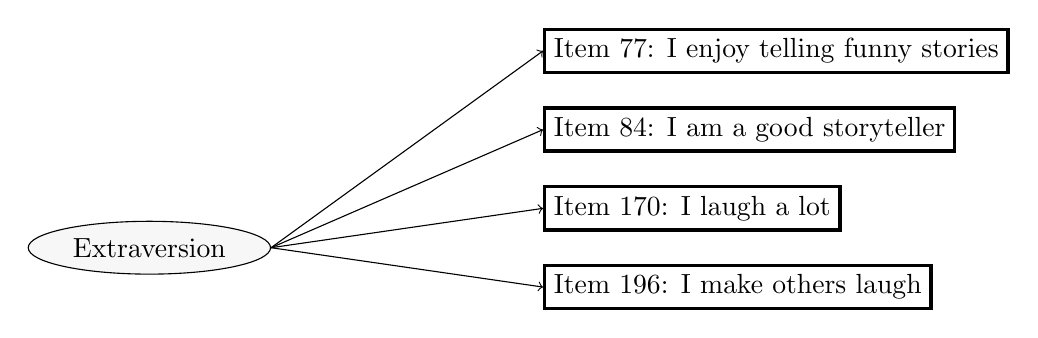
\begin{tikzpicture}[
      squarednode/.style={rectangle, draw=black, very thick, minimum size=5mm},
      arrow/.style = {thick}
    ]
    \usetikzlibrary{shapes.geometric}

    %Nodes
    \node[ellipse, draw,fill=gray!6] at (-1,-1) (latent) {Extraversion};
    \node[squarednode,right=2cm of latent,yshift=0.5cm] at (2,1) (Item77) {Item 77: I enjoy telling funny stories}; 
    \node[squarednode,right=2cm of latent,yshift=0.5cm] at (2,0) (Item84) {Item 84: I am a good storyteller};
    \node[squarednode,right=2cm of latent,yshift=0.5cm] at (2, -1) (Item170) {Item 170: I laugh a lot};
    \node[squarednode,right=2cm of latent,yshift=0.5cm] at (2,-2) (Item196) {Item 196: I make others laugh};
    
    %%Arrows
    \draw[->] (latent.east) -- (Item77.west);
    \draw[->] (latent.east) -- (Item84.west);
    \draw[->] (latent.east) -- (Item170.west);
    \draw[->] (latent.east) -- (Item196.west);

\end{tikzpicture}}

\vspace{5mm}

    \begin{itemize}
        \item Items are dependent variables, caused by the factor!
        \item Latent variable `extraversion' explains item correlations:\\
        The factor is the reason for the covariances/correlations.
    \end{itemize}

\end{frame}

% Slide 6
\begin{frame}{Reflective measurement model}

    \scalebox{0.6}{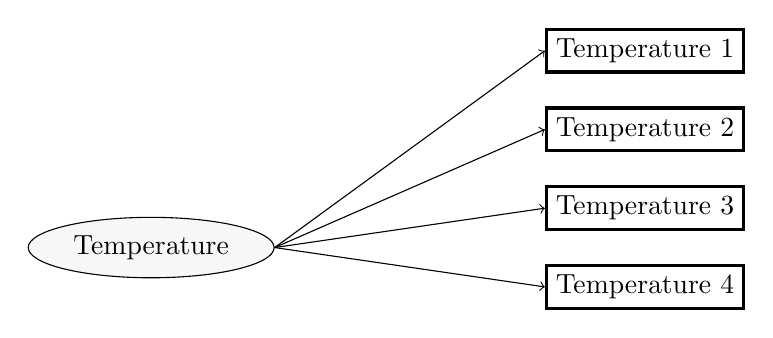
\begin{tikzpicture}[
      squarednode/.style={rectangle, draw=black, very thick, minimum size=5mm},
      arrow/.style = {thick}
    ]
    \usetikzlibrary{shapes.geometric}

    %Nodes
    \node[ellipse, draw,fill=gray!6] at (-1,-1) (latent) {Temperature};
    \node[squarednode,right=2cm of latent,yshift=0.5cm] at (2,1) (T1) {Temperature 1}; 
    \node[squarednode,right=2cm of latent,yshift=0.5cm] at (2,0) (T2) {Temperature 2};
    \node[squarednode,right=2cm of latent,yshift=0.5cm] at (2, -1) (T3) {Temperature 3};
    \node[squarednode,right=2cm of latent,yshift=0.5cm] at (2,-2) (T4) {Temperature 4};
    
    %%Arrows
    \draw[->] (latent.east) -- (T1.west);
    \draw[->] (latent.east) -- (T2.west);
    \draw[->] (latent.east) -- (T3.west);
    \draw[->] (latent.east) -- (T4.west);

    \end{tikzpicture}} 

\vspace{5mm}

Note: \\
Thermometer readings are the dependent variables, \\
caused by the temperature!

\end{frame}

% Slide 7
\begin{frame}{Reflective measurement model}

    \scalebox{0.6}{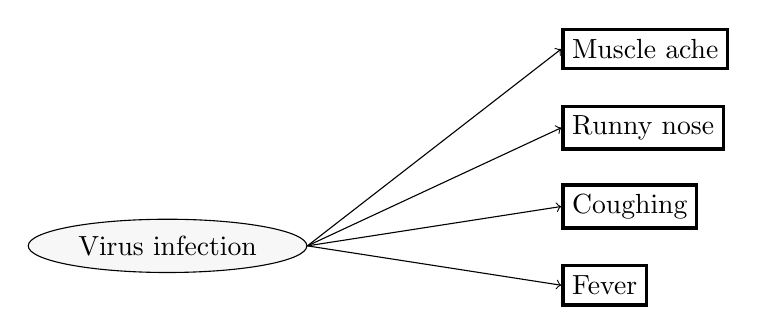
\begin{tikzpicture}[
      squarednode/.style={rectangle, draw=black, very thick, minimum size=5mm},
      arrow/.style = {thick}
    ]
    \usetikzlibrary{shapes.geometric}

    %Nodes
    \node[ellipse, draw,fill=gray!6] at (-1,-1) (latent) {Virus infection};
    \node[squarednode,right=2cm of latent,yshift=0.5cm] at (2,1) (V1) {Muscle ache}; 
    \node[squarednode,right=2cm of latent,yshift=0.5cm] at (2,0) (V2) {Runny nose};
    \node[squarednode,right=2cm of latent,yshift=0.5cm] at (2, -1) (V3) {Coughing};
    \node[squarednode,right=2cm of latent,yshift=0.5cm] at (2,-2) (V4) {Fever};
    
    %%Arrows
    \draw[->] (latent.east) -- (V1.west);
    \draw[->] (latent.east) -- (V2.west);
    \draw[->] (latent.east) -- (V3.west);
    \draw[->] (latent.east) -- (V4.west);

    \end{tikzpicture}}

\vspace{5mm}

Note: \\
symptoms are the dependent variables, \\
caused by the virus infection!

\end{frame}
%------------------------------------------------------------------------------%
%
%\subsection*{Formative}
%------------------------------------------------------------------------------%
%
% Slide 8+9
\begin{frame}{Formative measurement model}

If formative measurement model:

\vspace{5mm}

    \scalebox{0.6}{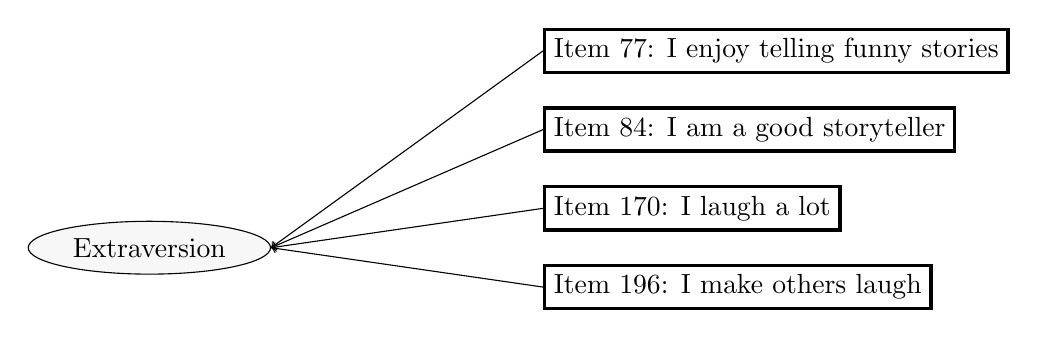
\begin{tikzpicture}[
      squarednode/.style={rectangle, draw=black, very thick, minimum size=5mm},
      arrow/.style = {thick}
    ]
    \usetikzlibrary{shapes.geometric}

    %Nodes
    \node[ellipse, draw,fill=gray!6] at (-1,-1) (latent) {Extraversion};
    \node[squarednode,right=2cm of latent,yshift=0.5cm] at (2,1) (Item77) {Item 77: I enjoy telling funny stories}; 
    \node[squarednode,right=2cm of latent,yshift=0.5cm] at (2,0) (Item84) {Item 84: I am a good storyteller};
    \node[squarednode,right=2cm of latent,yshift=0.5cm] at (2, -1) (Item170) {Item 170: I laugh a lot};
    \node[squarednode,right=2cm of latent,yshift=0.5cm] at (2,-2) (Item196) {Item 196: I make others laugh};
    
    %%Arrows
    \draw[->] (Item77.west) -- (latent.east);
    \draw[->] (Item84.west) -- (latent.east);
    \draw[->] (Item170.west) -- (latent.east);
    \draw[->] (Item196.west) -- (latent.east);

    \end{tikzpicture}}

\vspace{5mm}

Note: 
\begin{itemize}
	\item Extraversion is the dependent variable, predicted by the items.
	\item \textbf{Extraversion is \textit{defined} as a (weighted) sum of the items:}\\
	This is not a testable measurement model, but a definition.
\end{itemize}


\end{frame}
%------------------------------------------------------------------------------%
%
% Slide 10
\begin{frame}{Formative measurement model}

    \scalebox{0.6}{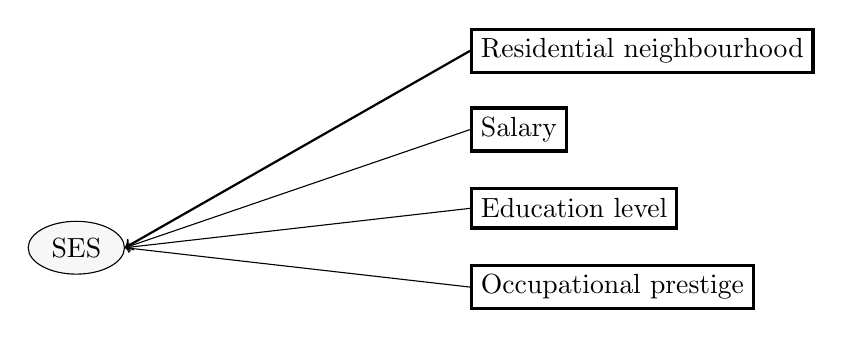
\begin{tikzpicture}[
      squarednode/.style={rectangle, draw=black, very thick, minimum size=5mm},
      arrow/.style = {thick}
    ]
    \usetikzlibrary{shapes.geometric}

    %Nodes
    \node[ellipse, draw,fill=gray!6] at (-1,-1) (latent) {SES};
    \node[squarednode,right=2cm of latent,yshift=0.5cm] at (2,1) (S1) {Residential neighbourhood}; 
    \node[squarednode,right=2cm of latent,yshift=0.5cm] at (2,0) (S2) {Salary};
    \node[squarednode,right=2cm of latent,yshift=0.5cm] at (2, -1) (S3) {Education level};
    \node[squarednode,right=2cm of latent,yshift=0.5cm] at (2,-2) (S4) {Occupational prestige};
    
    %%Arrows
    \draw[->,thick] (S1.west) -- (latent.east);
    \draw[->] (S2.west) -- (latent.east);
    \draw[->] (S3.west) -- (latent.east);
    \draw[->] (S4.west) -- (latent.east);

    \end{tikzpicture}} 

\vspace{5mm}

Note: \\
SES is defined as a (weighted) sum of the items.

\end{frame}
%------------------------------------------------------------------------------%
%
\subsection*{Sum scores}
%------------------------------------------------------------------------------%
%
% Slide 11
%\begin{frame}{Intermezzo}
\begin{frame}{Interesting read}

Interesting read on theory \& latent variables: 

\vspace{5mm}

Borsboom, D., Mellenbergh, G.J., \& Van Heerden, J. (2003). The theoretical status of latent variables. \emph{Psychological review, 110}(2), 203.  
    
\end{frame}

% % Slide 11
% \begin{frame}{Sum scores: Types}
% 		\begin{itemize}
% 			\item Sum score: Sum all the item scores together.\\
% 			In R: rowSums(data).\\
% 			\item Average sum score: Take mean of the sum score.\\
% 			In R: mean(rowSums(data)) \\
% 			\item Weighted average sum score: Use factor loadings as weights.
% 		\end{itemize}
% 
% \vspace{5mm}
% 
% In first two, weights are 1 and 0 (items load or not),\\
% assumes equal weights (for items that load on the factor).\\
% Is good strategy in case of calculating Cronbach's alpha.
% 
% \end{frame}
% %------------------------------------------------------------------------------%
% %
% %% Slide 12 
% %
% %\begin{lstlisting}[language=R]
% %
% %# To sum over all items
% %rowSums(data)  
% %
% %# To take the mean of items
% %mean(rowSums(data)) 
% %
% %\end{lstlisting}
% %------------------------------------------------------------------------------%
% %
% %% Slide 13
% %\begin{frame}{Sum scores}
% %
% %Sum scores can be consistent with both reflective and formative measurement models. \vspace{5mm}
% %
% %
% %    \scalebox{0.6}{\begin{tikzpicture}[
% %      squarednode/.style={rectangle, draw=black, very thick, minimum size=5mm},
% %      arrow/.style = {thick}
% %    ]
% %    \usetikzlibrary{shapes.geometric}
% %
% %    %Nodes
% %    \node[ellipse, draw,fill=gray!6] at (-1,-1) (latent) {Extraversion};
% %    \node[squarednode,right=2cm of latent,yshift=0.5cm] at (3,1) (Item77) {Item 77: I enjoy telling funny stories}; 
% %    \node[squarednode,right=2cm of latent,yshift=0.5cm] at (3,0) (Item84) {Item 84: I am a good storyteller};
% %    \node[squarednode,right=2cm of latent,yshift=0.5cm] at (3, -1) (Item170) {Item 170: I laugh a lot};
% %    \node[squarednode,right=2cm of latent,yshift=0.5cm] at (3,-2) (Item196) {Item 196: I make others laugh};
% %    
% %    %%Arrows
% %    \draw[->] (latent.east) -- (Item77.west);
% %    \draw[->] (latent.east) -- (Item84.west);
% %    \draw[->] (latent.east) -- (Item170.west);
% %    \draw[->] (latent.east) -- (Item196.west);
% %
% %    \end{tikzpicture}} 
% %
% %    \scalebox{0.6}{\begin{tikzpicture}[
% %      squarednode/.style={rectangle, draw=black, very thick, minimum size=5mm},
% %      arrow/.style = {thick}
% %    ]
% %    \usetikzlibrary{shapes.geometric}
% %
% %    %Nodes
% %    \node[ellipse, draw,fill=gray!6] at (-1,-1) (latent) {Extraversion};
% %    \node[squarednode,right=2cm of latent,yshift=0.5cm] at (3,1) (Item77) {Item 77: I enjoy telling funny stories}; 
% %    \node[squarednode,right=2cm of latent,yshift=0.5cm] at (3,0) (Item84) {Item 84: I am a good storyteller};
% %    \node[squarednode,right=2cm of latent,yshift=0.5cm] at (3, -1) (Item170) {Item 170: I laugh a lot};
% %    \node[squarednode,right=2cm of latent,yshift=0.5cm] at (3,-2) (Item196) {Item 196: I make others laugh};
% %    
% %    %%Arrows
% %    \draw[<-] (latent.east) -- (Item77.west);
% %    \draw[<-] (latent.east) -- (Item84.west);
% %    \draw[<-] (latent.east) -- (Item170.west);
% %    \draw[<-] (latent.east) -- (Item196.west);
% %
% %    \end{tikzpicture}} 
% %\vspace{5mm}
% %\textbf{But... each item gets the same weight!}
% %
% %\end{frame}
% %------------------------------------------------------------------------------%
% %
% % Slide 14 and slide 15
% \begin{frame}{Sum scores as a formative measurement model}
% 
%     \scalebox{0.6}{\begin{tikzpicture}[
%       squarednode/.style={rectangle, draw=black, very thick, minimum size=5mm},
%       arrow/.style = {thick}
%     ]
%     \usetikzlibrary{shapes.geometric}
% 
%     %Nodes
%     \node[ellipse, draw,fill=gray!6] at (-1,-1) (latent) {Extraversion};
%     \node[squarednode,right=2cm of latent,yshift=0.5cm] at (3,1) (Item77) {Item 77: I enjoy telling funny stories}; 
%     \node[squarednode,right=2cm of latent,yshift=0.5cm] at (3,0) (Item84) {Item 84: I am a good storyteller};
%     \node[squarednode,right=2cm of latent,yshift=0.5cm] at (3, -1) (Item170) {Item 170: I laugh a lot};
%     \node[squarednode,right=2cm of latent,yshift=0.5cm] at (3,-2) (Item196) {Item 196: I make others laugh};
%     
%     %%Arrows
%     \draw[<-] (latent.east) -- (Item77.west)node[midway,above left] {=};
%     \draw[<-] (latent.east) -- (Item84.west)node[midway,above left] {=};
%     \draw[<-] (latent.east) -- (Item170.west)node[midway,above left] {=};
%     \draw[<-] (latent.east) -- (Item196.west)node[midway,above left] {=};
% 
%     \end{tikzpicture}} 
% 
% \vspace{5mm}
% 
% Each item is 
% \begin{itemize}
% 	\item equally important in defining the latent variable.
% 	\item equally reflective of the latent variable.
% \end{itemize}
% 
% \end{frame}
% %------------------------------------------------------------------------------%
% %
% %% Slide 16
% %
% %\begin{lstlisting}[language=R]{Factor Scores: R} % Geeft nu geen header....
% %
% %# Model statement
% %model.CFA <- 
% %    'Extraversion=~Item77+Item84+Item170+Item196'
% %
% %# Fit the model 
% %fit.CFA <- cfa(model.CFA,
% %           data=data_sapi,
% %           missing='fiml',
% %           fixed.x=F) 
% %
% %# Model output
% %summary(fit.CFA)
% %
% %\end{lstlisting}
% 
% 
% % Slide 17
% \begin{frame}{Factor Scores}
%     
% 
%      \scalebox{0.6}{\begin{tikzpicture}[
%       squarednode/.style={rectangle, draw=black, very thick, minimum size=5mm},
%       arrow/.style = {thick}
%     ]
%     \usetikzlibrary{shapes.geometric}
% 
%     %Nodes
%     \node[ellipse, draw,fill=gray!6] at (-1,-1) (latent) {Extraversion};
%     \node[squarednode,right=2cm of latent,yshift=0.5cm] at (3,1) (Item77) {Item 77: I enjoy telling funny stories}; 
%     \node[squarednode,right=2cm of latent,yshift=0.5cm] at (3,0) (Item84) {Item 84: I am a good storyteller};
%     \node[squarednode,right=2cm of latent,yshift=0.5cm] at (3, -1) (Item170) {Item 170: I laugh a lot};
%     \node[squarednode,right=2cm of latent,yshift=0.5cm] at (3,-2) (Item196) {Item 196: I make others laugh};
%     
%     %%Arrows
%     \draw[->] (latent.east) -- (Item77.west) node[midway,above left] {1.00};
%     \draw[->] (latent.east) -- (Item84.west)node[above left] {0.708};
%     \draw[->] (latent.east) -- (Item170.west)node[above left] {0.567};
%     \draw[->] (latent.east) -- (Item196.west)node[above left] {0.742};
% 
%     \end{tikzpicture}} 
% 
% 
% \vspace{5mm}
% 
% \begin{itemize}
% 	\item The factor loadings are unequal when estimated with factor analysis.
% 	\item Items do not seem to be equally reflective of Extraversion.
% \end{itemize}
% 
% \end{frame}
%% Comment Slide 17
%% With factor analysis you can determine the extent to which items designed to measure a particular factor (in this case extraversion) actually do so. 
%% It is the ‘true’ correlation between an indicator and a factor 
%% So, every factor (in this case Extraversion) is a weighted sum of the items 
% Vraag: dus dan weighted sum score niet formative maar reflective?
% 
% %% Slide 18
% %
% %\begin{lstlisting}[language=R]{Test assumption of equal loadings}
% %
% %# Model specification
% %model.CFA.equal <- '
% % Extraversion=~Q77+a*Q84+Q170+b*Q196
% %'
% %
% %# Fit model
% %fit.CFA.equal <- cfa(model.CFA_equal,
% %                data=data_sapi,
% %                missing='fiml',
% %                fixed.x=F) 
% %
% %# Wald test
% %lavTestWald(fit.CFA.equal, constraints = 'a==b')
% %
% %\end{lstlisting}
%------------------------------------------------------------------------------%
%
%% Slide 19
%------------------------------------------------------------------------------%
%
%\subsection*{EFA vs CFA}
%------------------------------------------------------------------------------%
%
% Slide 28
\begin{frame}

\begin{center}
   \Huge Confirmatory or exploratory?
\end{center}

\end{frame}
%------------------------------------------------------------------------------%
%
% Slide 29
\begin{frame}{Two sub-scales of extraversion}

    \scalebox{0.6}{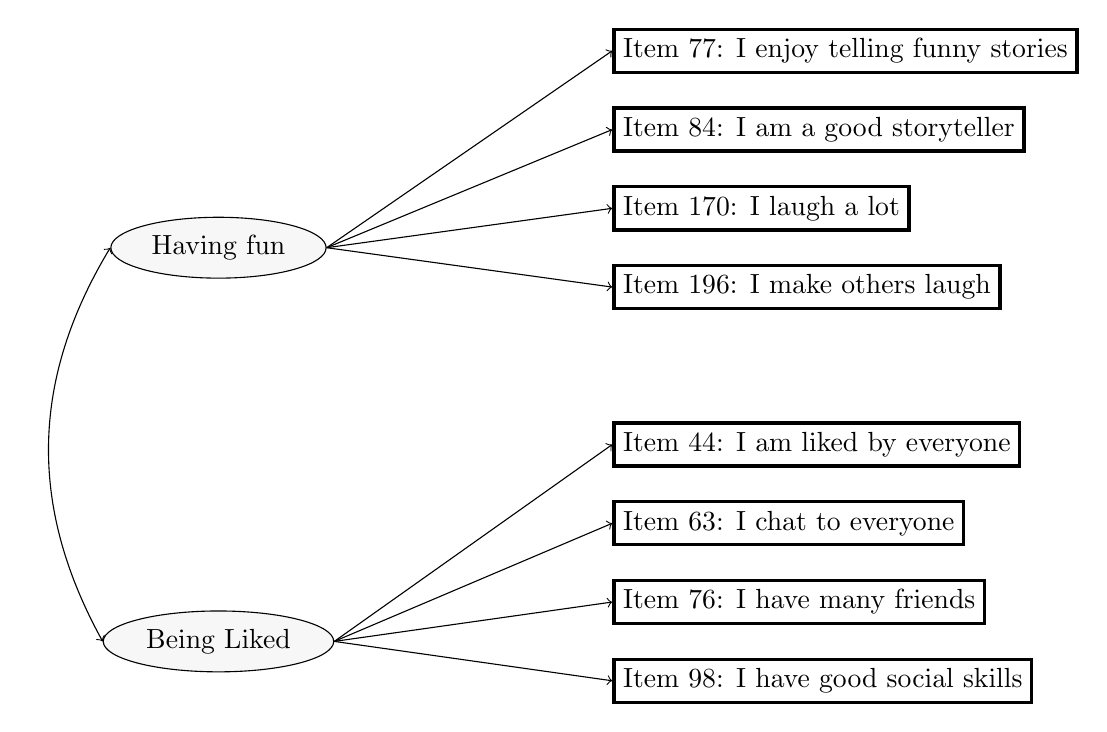
\begin{tikzpicture}[
  squarednode/.style={rectangle, draw=black, very thick, minimum size=5mm},
  arrow/.style = {thick}
]
    \usetikzlibrary{shapes.geometric}

    %Nodes
    \node[ellipse, draw,fill=gray!6] at (-1,3) (latent) {Having fun};
    \node[squarednode,right=2cm of latent,yshift=0.5cm] at (2,5) (Item77) {Item 77: I enjoy telling funny stories}; 
    \node[squarednode,right=2cm of latent,yshift=0.5cm] at (2,4) (Item84) {Item 84: I am a good storyteller};
    \node[squarednode,right=2cm of latent,yshift=0.5cm] at (2,3) (Item170) {Item 170: I laugh a lot};
    \node[squarednode,right=2cm of latent,yshift=0.5cm] at (2,2) (Item196) {Item 196: I make others laugh};
    
    %%Arrows
    \draw[->] (latent.east) -- (Item77.west);
    \draw[->] (latent.east) -- (Item84.west);
    \draw[->] (latent.east) -- (Item170.west);
    \draw[->] (latent.east) -- (Item196.west);


    %Nodes
    \node[ellipse, draw,fill=gray!6] at (-1,-2) (liked) {Being Liked};
    \node[squarednode,right=2cm of liked,yshift=0.5cm] at (2,0) (Item44) {Item 44: I am liked by everyone}; 
    \node[squarednode,right=2cm of liked,yshift=0.5cm] at (2,-1) (Item63) {Item 63: I chat to everyone};
    \node[squarednode,right=2cm of liked,yshift=0.5cm] at (2, -2) (Item76) {Item 76: I have many friends};
    \node[squarednode,right=2cm of liked,yshift=0.5cm] at (2,-3) (Item98) {Item 98: I have good social skills};
    
    %%Arrows
    \draw[->] (liked.east) -- (Item44.west);
    \draw[->] (liked.east) -- (Item63.west);
    \draw[->] (liked.east) -- (Item76.west);
    \draw[->] (liked.east) -- (Item98.west);
    
    \path[<->] (liked.west) edge [bend left] (latent.west);

    \end{tikzpicture}} \\

\end{frame}
%------------------------------------------------------------------------------%
%
% Slide 31
\begin{frame}{EFA: all loadings including cross-loadings}

    \scalebox{0.6}{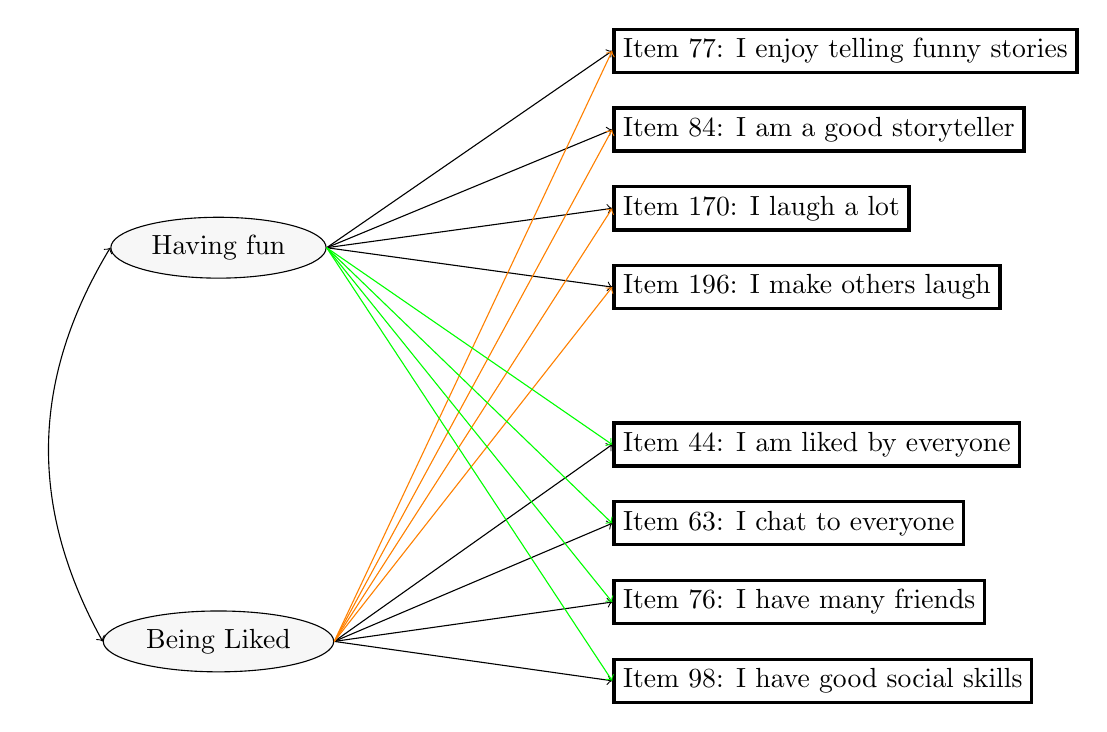
\begin{tikzpicture}[
  squarednode/.style={rectangle, draw=black, very thick, minimum size=5mm},
  arrow/.style = {thick}
]
    \usetikzlibrary{shapes.geometric}

    %Nodes
    \node[ellipse, draw,fill=gray!6] at (-1,3) (latent) {Having fun};
    \node[squarednode,right=2cm of latent,yshift=0.5cm] at (2,5) (Item77) {Item 77: I enjoy telling funny stories}; 
    \node[squarednode,right=2cm of latent,yshift=0.5cm] at (2,4) (Item84) {Item 84: I am a good storyteller};
    \node[squarednode,right=2cm of latent,yshift=0.5cm] at (2,3) (Item170) {Item 170: I laugh a lot};
    \node[squarednode,right=2cm of latent,yshift=0.5cm] at (2,2) (Item196) {Item 196: I make others laugh};
    
    %%Arrows
    \draw[->] (latent.east) -- (Item77.west);
    \draw[->] (latent.east) -- (Item84.west);
    \draw[->] (latent.east) -- (Item170.west);
    \draw[->] (latent.east) -- (Item196.west);
    
    %Nodes
    \node[ellipse, draw,fill=gray!6] at (-1,-2) (liked) {Being Liked};
    \node[squarednode,right=2cm of liked,yshift=0.5cm] at (2,0) (Item44) {Item 44: I am liked by everyone}; 
    \node[squarednode,right=2cm of liked,yshift=0.5cm] at (2,-1) (Item63) {Item 63: I chat to everyone};
    \node[squarednode,right=2cm of liked,yshift=0.5cm] at (2, -2) (Item76) {Item 76: I have many friends};
    \node[squarednode,right=2cm of liked,yshift=0.5cm] at (2,-3) (Item98) {Item 98: I have good social skills};
    
    %%Arrows
    \draw[->] (liked.east) -- (Item44.west);
    \draw[->] (liked.east) -- (Item63.west);
    \draw[->] (liked.east) -- (Item76.west);
    \draw[->] (liked.east) -- (Item98.west);
    
    \path[<->] (liked.west) edge [bend left] (latent.west);
    
    \draw[orange,->] (liked.east) -- (Item77.west);
    \draw[orange,->] (liked.east) -- (Item84.west);
    \draw[orange,->] (liked.east) -- (Item170.west);
    \draw[orange,->] (liked.east) -- (Item196.west);
    
    \draw[green,->] (latent.east) -- (Item44.west);
    \draw[green,->] (latent.east) -- (Item63.west);
    \draw[green,->] (latent.east) -- (Item76.west);
    \draw[green,->] (latent.east) -- (Item98.west);

    \end{tikzpicture}} 

\end{frame}
%------------------------------------------------------------------------------%
%
% Slide 30
\begin{frame}{CFA: only hypothesized loadings}
	
	\scalebox{0.6}{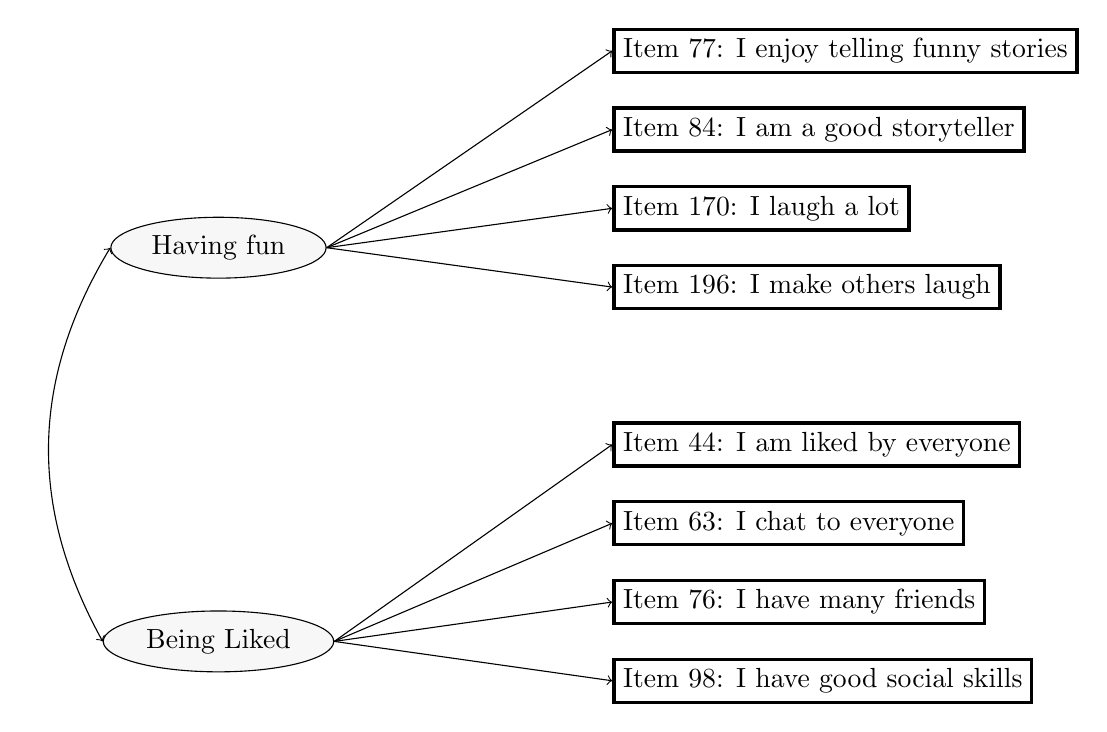
\begin{tikzpicture}[
			squarednode/.style={rectangle, draw=black, very thick, minimum size=5mm},
			arrow/.style = {thick}
			]
			\usetikzlibrary{shapes.geometric}
			
			%Nodes
			\node[ellipse, draw,fill=gray!6] at (-1,3) (latent) {Having fun};
			\node[squarednode,right=2cm of latent,yshift=0.5cm] at (2,5) (Item77) {Item 77: I enjoy telling funny stories}; 
			\node[squarednode,right=2cm of latent,yshift=0.5cm] at (2,4) (Item84) {Item 84: I am a good storyteller};
			\node[squarednode,right=2cm of latent,yshift=0.5cm] at (2,3) (Item170) {Item 170: I laugh a lot};
			\node[squarednode,right=2cm of latent,yshift=0.5cm] at (2,2) (Item196) {Item 196: I make others laugh};
			
			%%Arrows
			\draw[->] (latent.east) -- (Item77.west);
			\draw[->] (latent.east) -- (Item84.west);
			\draw[->] (latent.east) -- (Item170.west);
			\draw[->] (latent.east) -- (Item196.west);
			
			%Nodes
			\node[ellipse, draw,fill=gray!6] at (-1,-2) (liked) {Being Liked};
			\node[squarednode,right=2cm of liked,yshift=0.5cm] at (2,0) (Item44) {Item 44: I am liked by everyone}; 
			\node[squarednode,right=2cm of liked,yshift=0.5cm] at (2,-1) (Item63) {Item 63: I chat to everyone};
			\node[squarednode,right=2cm of liked,yshift=0.5cm] at (2, -2) (Item76) {Item 76: I have many friends};
			\node[squarednode,right=2cm of liked,yshift=0.5cm] at (2,-3) (Item98) {Item 98: I have good social skills};
			
			%%Arrows
			\draw[->] (liked.east) -- (Item44.west);
			\draw[->] (liked.east) -- (Item63.west);
			\draw[->] (liked.east) -- (Item76.west);
			\draw[->] (liked.east) -- (Item98.west);
			
			\path[<->] (liked.west) edge [bend left] (latent.west);
			
	\end{tikzpicture}} 
	
\end{frame}
%------------------------------------------------------------------------------%
%
%------------------------------------------------------------------------------%
\section{EFA in R}
%\subsection*{EFA in R}
%------------------------------------------------------------------------------%
%
%------------------------------------------------------------------------------%
\begin{frame}[fragile]{Step 1: Loading data into R}

\begin{knitrout}
\definecolor{shadecolor}{rgb}{0.969, 0.969, 0.969}\color{fgcolor}\begin{kframe}
\begin{alltt}
\hldef{data_sapi} \hlkwb{<-} \hlkwd{read.table}\hldef{(}\hlsng{"Sapi.txt"}\hldef{,} \hlkwc{header} \hldef{= T)}

\hldef{data_sapi[}\hlkwd{sapply}\hldef{(data_sapi,}
    \hlkwa{function}\hldef{(}\hlkwc{x}\hldef{)} \hlkwd{as.character}\hldef{(x)} \hlopt \hlkwd{c}\hldef{(}\hlsng{"-999"}\hldef{) )]} \hlkwb{<-} \hlnum{NA}
\end{alltt}
\end{kframe}
\end{knitrout}

\end{frame}
%------------------------------------------------------------------------------%
%
\begin{frame}[fragile]{Step 3: Draw your model}

\scalebox{0.6}{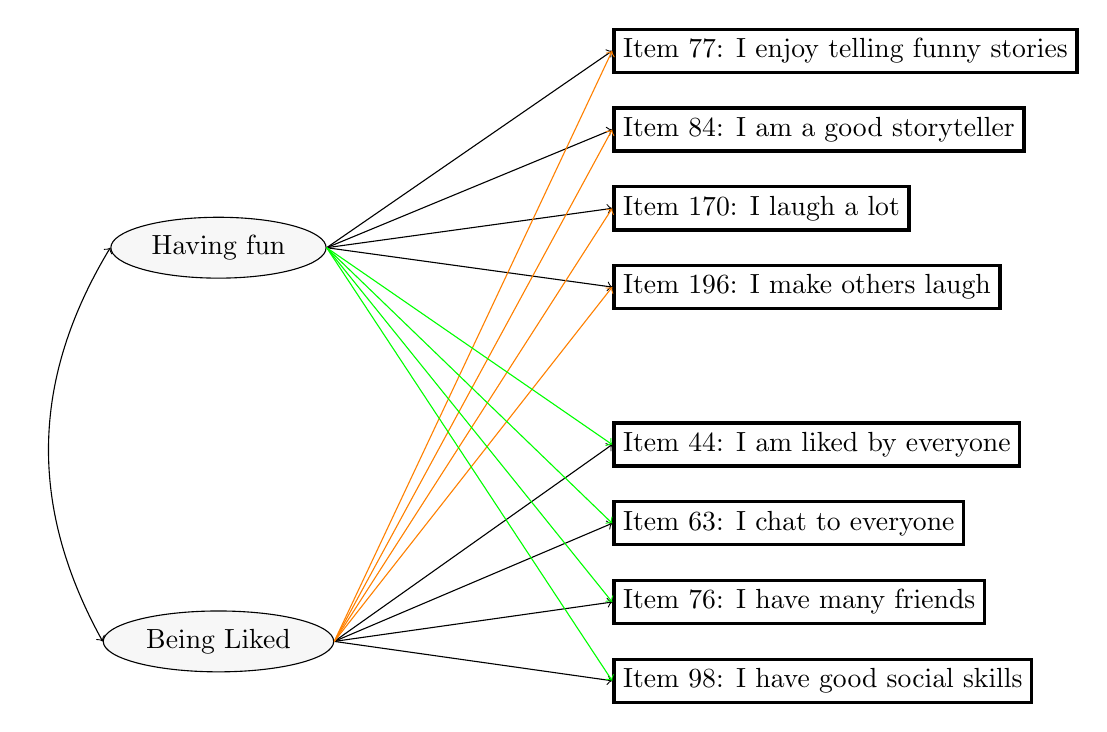
\begin{tikzpicture}[
  squarednode/.style={rectangle, draw=black, very thick, minimum size=5mm},
  arrow/.style = {thick}
]
    \usetikzlibrary{shapes.geometric}

    %Nodes
    \node[ellipse, draw,fill=gray!6] at (-1,3) (latent) {Having fun};
    \node[squarednode,right=2cm of latent,yshift=0.5cm] at (2,5) (Item77) {Item 77: I enjoy telling funny stories}; 
    \node[squarednode,right=2cm of latent,yshift=0.5cm] at (2,4) (Item84) {Item 84: I am a good storyteller};
    \node[squarednode,right=2cm of latent,yshift=0.5cm] at (2,3) (Item170) {Item 170: I laugh a lot};
    \node[squarednode,right=2cm of latent,yshift=0.5cm] at (2,2) (Item196) {Item 196: I make others laugh};
    
    %%Arrows
    \draw[->] (latent.east) -- (Item77.west);
    \draw[->] (latent.east) -- (Item84.west);
    \draw[->] (latent.east) -- (Item170.west);
    \draw[->] (latent.east) -- (Item196.west);
    
    %Nodes
    \node[ellipse, draw,fill=gray!6] at (-1,-2) (liked) {Being Liked};
    \node[squarednode,right=2cm of liked,yshift=0.5cm] at (2,0) (Item44) {Item 44: I am liked by everyone}; 
    \node[squarednode,right=2cm of liked,yshift=0.5cm] at (2,-1) (Item63) {Item 63: I chat to everyone};
    \node[squarednode,right=2cm of liked,yshift=0.5cm] at (2, -2) (Item76) {Item 76: I have many friends};
    \node[squarednode,right=2cm of liked,yshift=0.5cm] at (2,-3) (Item98) {Item 98: I have good social skills};
    
    %%Arrows
    \draw[->] (liked.east) -- (Item44.west);
    \draw[->] (liked.east) -- (Item63.west);
    \draw[->] (liked.east) -- (Item76.west);
    \draw[->] (liked.east) -- (Item98.west);
    
    \path[<->] (liked.west) edge [bend left] (latent.west);
    
    \draw[orange,->] (liked.east) -- (Item77.west);
    \draw[orange,->] (liked.east) -- (Item84.west);
    \draw[orange,->] (liked.east) -- (Item170.west);
    \draw[orange,->] (liked.east) -- (Item196.west);
    
    \draw[green,->] (latent.east) -- (Item44.west);
    \draw[green,->] (latent.east) -- (Item63.west);
    \draw[green,->] (latent.east) -- (Item76.west);
    \draw[green,->] (latent.east) -- (Item98.west);

    \end{tikzpicture}} 

\end{frame}
%------------------------------------------------------------------------------%
%
\begin{frame}[fragile]{Step 4: Specify EFA in lavaan (general case)}

In factor analysis (EFA and CFA):
\begin{itemize}
  \item $\,\to\,$ is latent variable definition (`is measured by'): $=\sim$ 
  \item $\xleftrightarrow{}$ is covariance. By default, factors are related. % So, no specification needed.
  \item In EFA: use $efa("efa")*$ in front of the latent variable / factor.
\end{itemize}

\begin{knitrout}
\definecolor{shadecolor}{rgb}{0.969, 0.969, 0.969}\color{fgcolor}\begin{kframe}
\begin{alltt}
\hlcom{# 1-factor model}
\hldef{f1} \hlkwb{<-} \hlsng{'
efa("efa")*f1 =~ y1 + y2 + y3 + ...
'}
\hlcom{# 2-factor model}
\hldef{f2} \hlkwb{<-} \hlsng{'
efa("efa")*f1 +
efa("efa")*f2 =~ y1 + y2 + y3 + ...
'}
\hlcom{# 3-factor model}
\hldef{f3} \hlkwb{<-} \hlsng{'
efa("efa")*f1 +
efa("efa")*f2 +
efa("efa")*f3 =~ y1 + y2 + y3 + ...
'}
\end{alltt}
\end{kframe}
\end{knitrout}

\end{frame}
%------------------------------------------------------------------------------%
%
% Slide 33-38
\begin{frame}[fragile]{Step 4: Specify our SAPI EFA model}

In factor analysis (EFA and CFA):
\begin{itemize}
  \item $\,\to\,$ is latent variable definition (`is measured by'): $=\sim$ 
  \item $\xleftrightarrow{}$ is covariance. By default, factors related. % So, no specification needed.
  \item Use $efa("efa")*$ in front of the latent variable / factor.
\end{itemize}

\begin{knitrout}
\definecolor{shadecolor}{rgb}{0.969, 0.969, 0.969}\color{fgcolor}\begin{kframe}
\begin{alltt}
\hlcom{# two-factor EFA}
\hldef{model.2EFA} \hlkwb{<-} \hlsng{"
 efa('block1')*Havingfun  =~ Q77 + Q84 + Q170 + Q196 + 
                              Q44 + Q63 + Q76  + Q98
 efa('block1')*Beingliked =~ Q77 + Q84 + Q170 + Q196 + 
                              Q44 + Q63 + Q76  + Q98
"}
\end{alltt}
\end{kframe}
\end{knitrout}

\end{frame}
%------------------------------------------------------------------------------%
%
\begin{frame}[fragile]{Step 5: Fit the model}

Use the cfa() function in lavaan.

\begin{knitrout}
\definecolor{shadecolor}{rgb}{0.969, 0.969, 0.969}\color{fgcolor}\begin{kframe}
\begin{alltt}
\hldef{fit_2EFA} \hlkwb{<-} \hlkwd{cfa}\hldef{(model.2EFA,} \hlkwc{data}\hldef{=data_sapi,}
                \hlkwc{missing}\hldef{=}\hlsng{'fiml'}\hldef{,} \hlkwc{fixed.x}\hldef{=F)}  \hlcom{# use FIML}
\hlcom{# Note: FIML will be discusses in the Missing Data lecture.}
\end{alltt}
\end{kframe}
\end{knitrout}
\end{frame}
%------------------------------------------------------------------------------%
%
\subsection*{EFA in R - Part 2}
%------------------------------------------------------------------------------%
%
\begin{frame}[fragile]{Step 5. Fit the EFA model: All code}

\begin{knitrout}
\definecolor{shadecolor}{rgb}{0.969, 0.969, 0.969}\color{fgcolor}\begin{kframe}
\begin{alltt}
\hlcom{# Data}
\hldef{data_sapi} \hlkwb{<-} \hlkwd{read.table}\hldef{(}\hlsng{"Sapi.txt"}\hldef{,} \hlkwc{header} \hldef{= T)}
\hldef{data_sapi[}\hlkwd{sapply}\hldef{(data_sapi,}
    \hlkwa{function}\hldef{(}\hlkwc{x}\hldef{)} \hlkwd{as.character}\hldef{(x)} \hlopt \hlkwd{c}\hldef{(}\hlsng{"-999"}\hldef{) )]} \hlkwb{<-} \hlnum{NA}

\hlcom{# Model: two-factor EFA}
\hldef{model.2EFA} \hlkwb{<-} \hlsng{"
 efa('block1')*Havingfun  =~ Q77 + Q84 + Q170 + Q196 + 
                              Q44 + Q63 + Q76  + Q98
 efa('block1')*Beingliked =~ Q77 + Q84 + Q170 + Q196 + 
                              Q44 + Q63 + Q76  + Q98
"}

\hlcom{# Fit model}
\hldef{fit_2EFA} \hlkwb{<-} \hlkwd{cfa}\hldef{(model.2EFA,} \hlkwc{data}\hldef{=data_sapi,}
                \hlkwc{missing}\hldef{=}\hlsng{'fiml'}\hldef{,} \hlkwc{fixed.x}\hldef{=F)}  \hlcom{# use FIML }
\end{alltt}
\end{kframe}
\end{knitrout}
\end{frame}
%------------------------------------------------------------------------------%
%
\begin{frame}[fragile]{Step 6: Plot the lavaan model in R}

\begin{knitrout}
\definecolor{shadecolor}{rgb}{0.969, 0.969, 0.969}\color{fgcolor}\begin{kframe}
\begin{alltt}
\hlkwa{if} \hldef{(}\hlopt{!}\hlkwd{require}\hldef{(}\hlsng{"lavaanPlot"}\hldef{))} \hlkwd{install.packages}\hldef{(}\hlsng{"lavaanPlot"}\hldef{)}
\hlkwd{library}\hldef{(lavaanPlot)}
\end{alltt}
\end{kframe}
\end{knitrout}
\begin{knitrout}
\definecolor{shadecolor}{rgb}{0.969, 0.969, 0.969}\color{fgcolor}\begin{kframe}
\begin{alltt}
\hlkwd{lavaanPlot}\hldef{(}\hlkwc{model} \hldef{= fit_2EFA,}
           \hlkwc{node_options} \hldef{=} \hlkwd{list}\hldef{(}\hlkwc{shape} \hldef{=} \hlsng{"box"}\hldef{,}
                               \hlkwc{fontname} \hldef{=} \hlsng{"Helvetica"}\hldef{),}
           \hlkwc{edge_options} \hldef{=} \hlkwd{list}\hldef{(}\hlkwc{color} \hldef{=} \hlsng{"grey"}\hldef{),}
           \hlkwc{coefs} \hldef{= T,}
           \hlkwc{stand} \hldef{= T,} \hlcom{# standardized }
           \hlkwc{covs} \hldef{= T)}
\end{alltt}
\end{kframe}
\end{knitrout}
\end{frame}
%------------------------------------------------------------------------------%
%
\begin{frame}[fragile]{Step 6: Plot the lavaan model in R Ctd.}

\begin{knitrout}
\definecolor{shadecolor}{rgb}{0.969, 0.969, 0.969}\color{fgcolor}\begin{kframe}
\begin{alltt}
\hlkwd{lavaanPlot}\hldef{(}\hlkwc{model} \hldef{= fit_2EFA,}
           \hlkwc{node_options} \hldef{=} \hlkwd{list}\hldef{(}\hlkwc{shape} \hldef{=} \hlsng{"box"}\hldef{,}
                               \hlkwc{fontname} \hldef{=} \hlsng{"Helvetica"}\hldef{),}
           \hlkwc{edge_options} \hldef{=} \hlkwd{list}\hldef{(}\hlkwc{color} \hldef{=} \hlsng{"grey"}\hldef{),}
           \hlkwc{coefs} \hldef{= T,} \hlkwc{stand} \hldef{= T,} \hlkwc{covs} \hldef{= T)}
\end{alltt}
\end{kframe}
\includegraphics[width=\maxwidth]{figure/unnamed-chunk-8-1} 
\end{knitrout}
\end{frame}
%------------------------------------------------------------------------------%
%
% \begin{frame}[fragile]{Step 7: Technical output (Part 1)}
% <<>>=
% lavInspect(fit_2EFA)[1]
% @
% \end{frame}
% %------------------------------------------------------------------------------%
% %
% \begin{frame}[fragile]{Step 7: Technical output (Part 2)}
% <<>>=
% lavInspect(fit_2EFA)[2:3]
% @
% \end{frame}
% %------------------------------------------------------------------------------%
% %
% \begin{frame}[fragile]{Step 7: Technical output (Part 3)}
% <<>>=
% lavInspect(fit_2EFA)[4:5] # Now, no beta, so only 5 matrices.
% @
% \end{frame}
% %------------------------------------------------------------------------------%
% %
\begin{frame}[fragile]{Step 9: Acquiring the summary}

\begin{knitrout}
\definecolor{shadecolor}{rgb}{0.969, 0.969, 0.969}\color{fgcolor}\begin{kframe}
\begin{alltt}
\hlkwd{summary}\hldef{(fit_2EFA)}

\hlkwd{parameterEstimates}\hldef{(fit_2EFA)}

\hlkwd{fitMeasures}\hldef{(fit_2EFA,} \hlkwd{c}\hldef{(}\hlsng{"chisq"}\hldef{,} \hlsng{"df"}\hldef{,} \hlsng{"pvalue"}\hldef{,}
                        \hlsng{"cfi"}\hldef{,} \hlsng{"tli"}\hldef{,}
                        \hlsng{"rmsea"}\hldef{,}\hlsng{"srmr"}\hldef{))}
\hlcom{# As an example, there are more.}
\end{alltt}
\end{kframe}
\end{knitrout}

\end{frame}
%------------------------------------------------------------------------------%
%
\begin{frame}[fragile]{Step 9: Acquiring the summary}

\begin{knitrout}
\definecolor{shadecolor}{rgb}{0.969, 0.969, 0.969}\color{fgcolor}\begin{kframe}
\begin{alltt}
\hlkwd{parameterEstimates}\hldef{(fit_2EFA)[}\hlnum{1}\hlopt{:}\hlnum{16}\hldef{,}\hlnum{1}\hlopt{:}\hlnum{5}\hldef{][,}\hlopt{-}\hlnum{4}\hldef{]}
\end{alltt}
\begin{verbatim}
##           lhs op  rhs    est
## 1   Havingfun =~  Q77  0.884
## 2   Havingfun =~  Q84  0.493
## 3   Havingfun =~ Q170  0.336
## 4   Havingfun =~ Q196  0.523
## 5   Havingfun =~  Q44 -0.163
## 6   Havingfun =~  Q63  0.014
## 7   Havingfun =~  Q76  0.031
## 8   Havingfun =~  Q98  0.085
## 9  Beingliked =~  Q77 -0.028
## 10 Beingliked =~  Q84  0.186
## 11 Beingliked =~ Q170  0.187
## 12 Beingliked =~ Q196  0.119
## 13 Beingliked =~  Q44  0.576
## 14 Beingliked =~  Q63  0.632
## 15 Beingliked =~  Q76  0.595
## 16 Beingliked =~  Q98  0.465
\end{verbatim}
\end{kframe}
\end{knitrout}

\end{frame}
%------------------------------------------------------------------------------%
%
%------------------------------------------------------------------------------%
\section{CFA in R} 
%\subsection*{CFA in R} 
%------------------------------------------------------------------------------%
%
%------------------------------------------------------------------------------%
\begin{frame}[fragile]{Step 1: Loading data into R}

\begin{knitrout}
\definecolor{shadecolor}{rgb}{0.969, 0.969, 0.969}\color{fgcolor}\begin{kframe}
\begin{alltt}
\hldef{data_sapi} \hlkwb{<-} \hlkwd{read.table}\hldef{(}\hlsng{"Sapi.txt"}\hldef{,} \hlkwc{header} \hldef{= T)}

\hldef{data_sapi[}\hlkwd{sapply}\hldef{(data_sapi,}
    \hlkwa{function}\hldef{(}\hlkwc{x}\hldef{)} \hlkwd{as.character}\hldef{(x)} \hlopt \hlkwd{c}\hldef{(}\hlsng{"-999"}\hldef{) )]} \hlkwb{<-} \hlnum{NA}
\end{alltt}
\end{kframe}
\end{knitrout}

\end{frame}
%------------------------------------------------------------------------------%
%
\begin{frame}[fragile]{Step 3: Draw your model}

\scalebox{0.6}{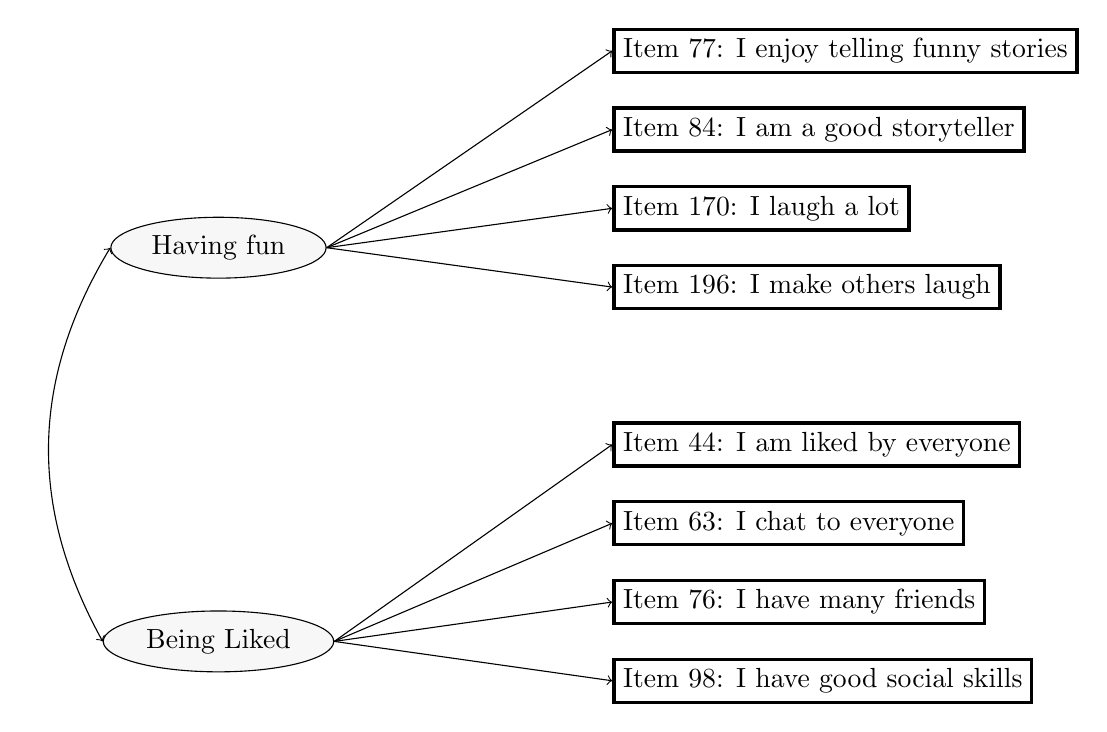
\begin{tikzpicture}[
			squarednode/.style={rectangle, draw=black, very thick, minimum size=5mm},
			arrow/.style = {thick}
			]
			\usetikzlibrary{shapes.geometric}
			
			%Nodes
			\node[ellipse, draw,fill=gray!6] at (-1,3) (latent) {Having fun};
			\node[squarednode,right=2cm of latent,yshift=0.5cm] at (2,5) (Item77) {Item 77: I enjoy telling funny stories}; 
			\node[squarednode,right=2cm of latent,yshift=0.5cm] at (2,4) (Item84) {Item 84: I am a good storyteller};
			\node[squarednode,right=2cm of latent,yshift=0.5cm] at (2,3) (Item170) {Item 170: I laugh a lot};
			\node[squarednode,right=2cm of latent,yshift=0.5cm] at (2,2) (Item196) {Item 196: I make others laugh};
			
			%%Arrows
			\draw[->] (latent.east) -- (Item77.west);
			\draw[->] (latent.east) -- (Item84.west);
			\draw[->] (latent.east) -- (Item170.west);
			\draw[->] (latent.east) -- (Item196.west);
			
			%Nodes
			\node[ellipse, draw,fill=gray!6] at (-1,-2) (liked) {Being Liked};
			\node[squarednode,right=2cm of liked,yshift=0.5cm] at (2,0) (Item44) {Item 44: I am liked by everyone}; 
			\node[squarednode,right=2cm of liked,yshift=0.5cm] at (2,-1) (Item63) {Item 63: I chat to everyone};
			\node[squarednode,right=2cm of liked,yshift=0.5cm] at (2, -2) (Item76) {Item 76: I have many friends};
			\node[squarednode,right=2cm of liked,yshift=0.5cm] at (2,-3) (Item98) {Item 98: I have good social skills};
			
			%%Arrows
			\draw[->] (liked.east) -- (Item44.west);
			\draw[->] (liked.east) -- (Item63.west);
			\draw[->] (liked.east) -- (Item76.west);
			\draw[->] (liked.east) -- (Item98.west);
			
			\path[<->] (liked.west) edge [bend left] (latent.west);
			
	\end{tikzpicture}} 

\end{frame}
%------------------------------------------------------------------------------%
%
\begin{frame}[fragile]{Step 4: Specify CFA in lavaan (general case)}

\begin{itemize}
  \item $\,\to\,$ is latent variable definition (`is measured by'): $=\sim$ 
  \item $\xleftrightarrow{}$ is covariance. By default, factors are related. % So, no specification needed.
\end{itemize}

\begin{knitrout}
\definecolor{shadecolor}{rgb}{0.969, 0.969, 0.969}\color{fgcolor}\begin{kframe}
\begin{alltt}
\hlcom{# k-factor model}
\hldef{model.kCFA} \hlkwb{<-} \hlsng{'
latent variable_1 =~ indicator11 + indicator12 + ...
latent variable_2 =~ indicator21 + indicator22 + ...
...
latent variable_k =~ indicatork1 + indicatork2 + ...
'}
\end{alltt}
\end{kframe}
\end{knitrout}

\end{frame}
%------------------------------------------------------------------------------%
%
% Slide 39-44
\begin{frame}[fragile]{Step 4: Specify our SAPI CFA model}

CFA: Only hypothesized loadings.\\
CFA vs EFA: force cross-loadings to zero.

\vspace{5mm}

In lavaan: \\
one can fix loadings to zero, BUT instead:\\
let manifest variables only appear in the equation of their factor.

\vspace{5mm}

\begin{knitrout}
\definecolor{shadecolor}{rgb}{0.969, 0.969, 0.969}\color{fgcolor}\begin{kframe}
\begin{alltt}
\hlcom{# two-factor CFA}
\hldef{model.2CFA} \hlkwb{<-} \hlsng{"
 Havingfun  =~ Q77 + Q84 + Q170 + Q196 
 Beingliked =~ Q44 + Q63 + Q76  + Q98
"}
\end{alltt}
\end{kframe}
\end{knitrout}

\end{frame}
%------------------------------------------------------------------------------%
%
\begin{frame}[fragile]{Step 5: Fit the model}

Use the cfa() function in lavaan.

\begin{knitrout}
\definecolor{shadecolor}{rgb}{0.969, 0.969, 0.969}\color{fgcolor}\begin{kframe}
\begin{alltt}
\hldef{fit_2CFA} \hlkwb{<-} \hlkwd{cfa}\hldef{(model.2CFA,} \hlkwc{data}\hldef{=data_sapi,}
                \hlkwc{missing}\hldef{=}\hlsng{'fiml'}\hldef{,} \hlkwc{fixed.x}\hldef{=F)}  \hlcom{# use FIML}
\hlcom{# Note: FIML will be discusses in the Missing Data lecture.}
\end{alltt}
\end{kframe}
\end{knitrout}
\end{frame}
%------------------------------------------------------------------------------%
%
\begin{frame}[fragile]{5. Fit the CFA model: All code}
\begin{knitrout}
\definecolor{shadecolor}{rgb}{0.969, 0.969, 0.969}\color{fgcolor}\begin{kframe}
\begin{alltt}
\hlcom{# Data}
\hldef{data_sapi} \hlkwb{<-} \hlkwd{read.table}\hldef{(}\hlsng{"Sapi.txt"}\hldef{,} \hlkwc{header} \hldef{= T)}
\hldef{data_sapi[}\hlkwd{sapply}\hldef{(data_sapi,}
    \hlkwa{function}\hldef{(}\hlkwc{x}\hldef{)} \hlkwd{as.character}\hldef{(x)} \hlopt \hlkwd{c}\hldef{(}\hlsng{"-999"}\hldef{) )]} \hlkwb{<-} \hlnum{NA}

\hlcom{# Model: two-factor CFA}
\hldef{model.2CFA} \hlkwb{<-} \hlsng{"
 Havingfun  =~ Q77 + Q84 + Q170 + Q196 
 Beingliked =~ Q44 + Q63 + Q76  + Q98
"}

\hlcom{# Fit model}
\hldef{fit_2CFA} \hlkwb{<-} \hlkwd{cfa}\hldef{(model.2CFA,} \hlkwc{data}\hldef{=data_sapi,}
                \hlkwc{missing}\hldef{=}\hlsng{'fiml'}\hldef{,} \hlkwc{fixed.x}\hldef{=F)}  \hlcom{# use FIML }
\end{alltt}
\end{kframe}
\end{knitrout}
\end{frame}
%------------------------------------------------------------------------------%
%
\begin{frame}[fragile]{Step 6: Plot the lavaan model in R}

\begin{knitrout}
\definecolor{shadecolor}{rgb}{0.969, 0.969, 0.969}\color{fgcolor}\begin{kframe}
\begin{alltt}
\hlkwa{if} \hldef{(}\hlopt{!}\hlkwd{require}\hldef{(}\hlsng{"lavaanPlot"}\hldef{))} \hlkwd{install.packages}\hldef{(}\hlsng{"lavaanPlot"}\hldef{)}
\hlkwd{library}\hldef{(lavaanPlot)}
\end{alltt}
\end{kframe}
\end{knitrout}
\begin{knitrout}
\definecolor{shadecolor}{rgb}{0.969, 0.969, 0.969}\color{fgcolor}\begin{kframe}
\begin{alltt}
\hlkwd{lavaanPlot}\hldef{(}\hlkwc{model} \hldef{= fit_2CFA,}
           \hlkwc{node_options} \hldef{=} \hlkwd{list}\hldef{(}\hlkwc{shape} \hldef{=} \hlsng{"box"}\hldef{,}
                               \hlkwc{fontname} \hldef{=} \hlsng{"Helvetica"}\hldef{),}
           \hlkwc{edge_options} \hldef{=} \hlkwd{list}\hldef{(}\hlkwc{color} \hldef{=} \hlsng{"grey"}\hldef{),}
           \hlkwc{coefs} \hldef{= T,}
           \hlkwc{stand} \hldef{= T,}
           \hlkwc{covs} \hldef{= T)}
\end{alltt}
\end{kframe}
\end{knitrout}
\end{frame}
%------------------------------------------------------------------------------%
%
\begin{frame}[fragile]{Step 6: Plot the lavaan model in R Ctd.}

\begin{knitrout}
\definecolor{shadecolor}{rgb}{0.969, 0.969, 0.969}\color{fgcolor}\begin{kframe}
\begin{alltt}
\hlkwd{lavaanPlot}\hldef{(}\hlkwc{model} \hldef{= fit_2CFA,}
           \hlkwc{node_options} \hldef{=} \hlkwd{list}\hldef{(}\hlkwc{shape} \hldef{=} \hlsng{"box"}\hldef{,}
                               \hlkwc{fontname} \hldef{=} \hlsng{"Helvetica"}\hldef{),}
           \hlkwc{edge_options} \hldef{=} \hlkwd{list}\hldef{(}\hlkwc{color} \hldef{=} \hlsng{"grey"}\hldef{),} \hlkwc{coefs} \hldef{= T,}
           \hlkwc{stand} \hldef{= T,} \hlkwc{covs} \hldef{= T)}
\end{alltt}
\end{kframe}
\includegraphics[width=\maxwidth]{figure/unnamed-chunk-18-1} 
\end{knitrout}
\end{frame}
%------------------------------------------------------------------------------%
%
% \begin{frame}[fragile]{Step 7: Technical output (Part 1)}
% <<>>=
% lavInspect(fit_2CFA)[1]
% @
% \end{frame}
% %------------------------------------------------------------------------------%
% %
% \begin{frame}[fragile]{Step 7: Technical output (Part 2)}
% <<>>=
% lavInspect(fit_2CFA)[2:3]
% @
% \end{frame}
% %------------------------------------------------------------------------------%
% %
% \begin{frame}[fragile]{Step 7: Technical output (Part 3)}
% <<>>=
% lavInspect(fit_2CFA)[4:5] # Now, no beta, so only 5 matrices.
% @
% \end{frame}
% %------------------------------------------------------------------------------%
% 
%------------------------------------------------------------------------------%
%
\subsection*{CFA in R - Part 2}
%------------------------------------------------------------------------------%
%
\begin{frame}[fragile]{Step 9: Acquiring the summary}

\begin{knitrout}
\definecolor{shadecolor}{rgb}{0.969, 0.969, 0.969}\color{fgcolor}\begin{kframe}
\begin{alltt}
\hlkwd{summary}\hldef{(fit_2CFA)}

\hlkwd{parameterEstimates}\hldef{(fit_2CFA)}

\hlkwd{fitMeasures}\hldef{(fit_2CFA,} \hlkwd{c}\hldef{(}\hlsng{"chisq"}\hldef{,} \hlsng{"df"}\hldef{,} \hlsng{"pvalue"}\hldef{,}
                        \hlsng{"cfi"}\hldef{,} \hlsng{"tli"}\hldef{,}
                        \hlsng{"rmsea"}\hldef{,}\hlsng{"srmr"}\hldef{))}
\hlcom{# As an example, there are more.}
\end{alltt}
\end{kframe}
\end{knitrout}

\begin{knitrout}
\definecolor{shadecolor}{rgb}{0.969, 0.969, 0.969}\color{fgcolor}\begin{kframe}
\begin{alltt}
\hlcom{#The factors scores for each subject can be required via:}
\hlkwd{predict}\hldef{(fit_2CFA)}
\end{alltt}
\end{kframe}
\end{knitrout}

\end{frame}
%------------------------------------------------------------------------------%
%
% Slide 45
\begin{frame}[fragile]{CFA: modification indices - lavaan commands}

Remark: Blending confirmatory and exploratory!\\
Make sure it makes sense!

\vspace{5mm}

In lavaan, modification indices can be requested
\begin{itemize}
  \item within the summary call:\\
\begin{knitrout}
\definecolor{shadecolor}{rgb}{0.969, 0.969, 0.969}\color{fgcolor}\begin{kframe}
\begin{alltt}
\hlkwd{summary}\hldef{(fit_2CFA,} \hlkwc{modindices} \hldef{=} \hlnum{TRUE}\hldef{)}
\end{alltt}
\end{kframe}
\end{knitrout}
  \item directly: \\
\begin{knitrout}
\definecolor{shadecolor}{rgb}{0.969, 0.969, 0.969}\color{fgcolor}\begin{kframe}
\begin{alltt}
\hlkwd{modindices}\hldef{(fit_2CFA,} \hlkwc{sort} \hldef{=} \hlnum{TRUE}\hldef{)}
\end{alltt}
\end{kframe}
\end{knitrout}
  \item for specific parameters, say, factor loadings:\\
\begin{knitrout}
\definecolor{shadecolor}{rgb}{0.969, 0.969, 0.969}\color{fgcolor}\begin{kframe}
\begin{alltt}
\hldef{mi} \hlkwb{<-} \hlkwd{modindices}\hldef{(fit)}
\hldef{mi[mi}\hlopt{$}\hldef{op} \hlopt{==} \hlsng{"=~"}\hldef{,]}
\end{alltt}
\end{kframe}
\end{knitrout}
\end{itemize}

Also, have a look at the lavTestScore() function.
%It is important to realize that the modindices() function will only consider fixed-to-zero parameters. If you have equality constraints in the model, and you wish to examine what happens if you release all (or some) of these equality constraints, use the lavTestScore() function.

\end{frame}
%------------------------------------------------------------------------------%
%
% Slide 46
\begin{frame}[fragile]{CFA: modification indices - interpretation}

%\includegraphics[width=\linewidth,height=0.5\textwidth,keepaspectratio]{images/slide46.png} 

\begin{knitrout}
\definecolor{shadecolor}{rgb}{0.969, 0.969, 0.969}\color{fgcolor}\begin{kframe}
\begin{alltt}
\hlcom{#modindices(fit, sort = TRUE, maximum.number = 7) # or:}
\hlkwd{modindices}\hldef{(fit_2CFA,} \hlkwc{sort} \hldef{=} \hlnum{TRUE}\hldef{)[}\hlnum{1}\hlopt{:}\hlnum{7}\hldef{,]} \hlcom{# first 7 rows}
\end{alltt}
\begin{verbatim}
##           lhs op  rhs     mi    epc sepc.lv sepc.all sepc.nox
## 51       Q170 ~~ Q196 36.273  0.138   0.138    0.271    0.271
## 38        Q77 ~~  Q84 35.431  0.194   0.194    0.305    0.305
## 46        Q84 ~~ Q196 31.126 -0.143  -0.143   -0.276   -0.276
## 45        Q84 ~~ Q170 20.426 -0.123  -0.123   -0.170   -0.170
## 50        Q84 ~~  Q98 16.530  0.092   0.092    0.156    0.156
## 35 Beingliked =~  Q84 13.085  0.552   0.234    0.222    0.222
## 39        Q77 ~~ Q170 12.876 -0.104  -0.104   -0.166   -0.166
\end{verbatim}
\end{kframe}
\end{knitrout}

\begin{itemize}
  \item mi: If parameter freely estimated, overall Chi-square statistic could decrease by approximately this amount.
  \item epc (= expected parameter change): Approximate value that a parameter is expected to attain.
\end{itemize}

\end{frame}
%------------------------------------------------------------------------------%
%
% Slide 49
\begin{frame}{CFA: modification indices - cross-loadings}

\textbf{Cross-loadings:} \vspace{5mm}

\includegraphics[width=\linewidth,height=0.5\textwidth,keepaspectratio]{images/slide49.png} 

\end{frame}
%------------------------------------------------------------------------------%
%
% Slide 48
\begin{frame}{CFA: modification indices - residual variances}

\textbf{Residual covariances:} \vspace{5mm}

\includegraphics[width=\linewidth,height=0.5\textwidth,keepaspectratio]{images/slide48.png} 

\end{frame}
%------------------------------------------------------------------------------%
%
% Slide 47
\begin{frame}{CFA: modification indices - be aware!}

\centering
\includegraphics[width=\linewidth,height=0.5\textwidth,keepaspectratio]{images/CapOnChanceMI.png}      

\end{frame}
%------------------------------------------------------------------------------%
%
% Slide 48
\begin{frame}[fragile]{CFA: modification indices - modification}

\begin{knitrout}
\definecolor{shadecolor}{rgb}{0.969, 0.969, 0.969}\color{fgcolor}\begin{kframe}
\begin{alltt}
\hlkwd{modindices}\hldef{(fit_2CFA,} \hlkwc{sort} \hldef{=} \hlnum{TRUE}\hldef{)[}\hlnum{1}\hldef{,]}
\end{alltt}
\begin{verbatim}
##     lhs op  rhs     mi   epc sepc.lv sepc.all sepc.nox
## 51 Q170 ~~ Q196 36.273 0.138   0.138    0.271    0.271
\end{verbatim}
\begin{alltt}
\hlcom{# Allow residuals of Q170 and Q196 to covary}
\end{alltt}
\end{kframe}
\end{knitrout}

\begin{knitrout}
\definecolor{shadecolor}{rgb}{0.969, 0.969, 0.969}\color{fgcolor}\begin{kframe}
\begin{alltt}
\hlcom{# Modified model: }
\hlcom{# two-factor CFA + residual covariance Q170 and Q196}
\hldef{model.2CFA_mod} \hlkwb{<-} \hlsng{"
 Havingfun  =~ Q77 + Q84 + Q170 + Q196 
 Beingliked =~ Q44 + Q63 + Q76  + Q98
 Q170 ~~ Q196
"}

\hlcom{# Fit model}
\hldef{fit_2CFA_mod} \hlkwb{<-} \hlkwd{cfa}\hldef{(model.2CFA_mod,} \hlkwc{data}\hldef{=data_sapi,}
                    \hlkwc{missing}\hldef{=}\hlsng{'fiml'}\hldef{,} \hlkwc{fixed.x}\hldef{=F)}  \hlcom{# use FIML }
\end{alltt}
\end{kframe}
\end{knitrout}

\end{frame}
%------------------------------------------------------------------------------%
%
% Slide 49
\begin{frame}[fragile]{CFA: modification indices - test modification}

\begin{knitrout}
\definecolor{shadecolor}{rgb}{0.969, 0.969, 0.969}\color{fgcolor}\begin{kframe}
\begin{alltt}
\hlkwd{anova}\hldef{(fit_2CFA, fit_2CFA_mod)[,}\hlopt{-}\hlkwd{c}\hldef{(}\hlnum{2}\hldef{,}\hlnum{3}\hldef{)]} \hlcom{# without AIC & BIC}
\end{alltt}
\begin{verbatim}
##              Df   Chisq Chisq diff   RMSEA Df diff Pr(>Chisq)    
## fit_2CFA_mod 18  88.738                                          
## fit_2CFA     19 124.170     35.432 0.18556       1  2.641e-09 ***
## ---
## Signif. codes:  0 '***' 0.001 '**' 0.01 '*' 0.05 '.' 0.1 ' ' 1
\end{verbatim}
\end{kframe}
\end{knitrout}

\begin{knitrout}
\definecolor{shadecolor}{rgb}{0.969, 0.969, 0.969}\color{fgcolor}\begin{kframe}
\begin{alltt}
\hlkwd{modindices}\hldef{(fit_2CFA,} \hlkwc{sort} \hldef{=} \hlnum{TRUE}\hldef{)[}\hlnum{1}\hldef{,]}
\end{alltt}
\begin{verbatim}
##     lhs op  rhs     mi   epc sepc.lv sepc.all sepc.nox
## 51 Q170 ~~ Q196 36.273 0.138   0.138    0.271    0.271
\end{verbatim}
\end{kframe}
\end{knitrout}

\end{frame}
%------------------------------------------------------------------------------%
%
% Slide 50
\begin{frame}[fragile]{CFA: modification indices - new parameter value}

\begin{knitrout}
\definecolor{shadecolor}{rgb}{0.969, 0.969, 0.969}\color{fgcolor}\begin{kframe}
\begin{alltt}
\hlkwd{parameterEstimates}\hldef{(fit_2CFA_mod)[}\hlnum{9}\hldef{,}\hlopt{-}\hlkwd{c}\hldef{(}\hlnum{5}\hldef{,}\hlnum{6}\hldef{,}\hlnum{7}\hldef{)]} \hlcom{# no se, z, and p}
\end{alltt}
\begin{verbatim}
##    lhs op  rhs   est ci.lower ci.upper
## 9 Q170 ~~ Q196 0.137    0.089    0.184
\end{verbatim}
\end{kframe}
\end{knitrout}

\begin{knitrout}
\definecolor{shadecolor}{rgb}{0.969, 0.969, 0.969}\color{fgcolor}\begin{kframe}
\begin{alltt}
\hlkwd{modindices}\hldef{(fit_2CFA,} \hlkwc{sort} \hldef{=} \hlnum{TRUE}\hldef{)[}\hlnum{1}\hldef{,}\hlnum{1}\hlopt{:}\hlnum{5}\hldef{]} \hlcom{# no sepc }
\end{alltt}
\begin{verbatim}
##     lhs op  rhs     mi   epc
## 51 Q170 ~~ Q196 36.273 0.138
\end{verbatim}
\end{kframe}
\end{knitrout}

\end{frame}
%------------------------------------------------------------------------------%
%
% Slide 51
\begin{frame}[fragile]{CFA: cross-loadings approximately zero}

\textbf{Problem:}
    \begin{itemize}
        \item Restricting cross-loadings to exactly zero can be too strict.
        \item Consequence: rejection of the model, model modifications that capitalise on chance.
    \end{itemize}

\textbf{(Possible) solution in Bayesian SEM (BSEM) \ blavaan:}
    \begin{itemize}
        \item Replace exact zero restrictions with approximate ones.
        \item Using Bayesian small-variance priors.
    \end{itemize}
\vspace{5mm}
\textbf{Interesting reading:}\\
$-$ Merkle, E. C., \& Rosseel, Y. (2018). blavaan: Bayesian Structural Equation Models via Parameter Expansion. Journal of Statistical Software, 85(4), 1–30. https://doi.org/10.18637/jss.v085.i04
\\
$-$ Muthén, B., \& Asparouhov, T. (2012). Bayesian structural equation modelling: A more flexible representation of substantive theory. Psychological Methods, 17(3), 313-335.
\end{frame}
%------------------------------------------------------------------------------%
%
%------------------------------------------------------------------------------%
%-----------------------------------------------------------
% SECTION 2
%
% Slide 52
\section{Scaling}
%\subsection*{Theory}
% \begin{frame}
% 
% \begin{center}
%     \Huge 2. Latent variable scale
% \end{center}
% 
% \end{frame}
%------------------------------------------------------------------------------%
%
%------------------------------------------------------------------------------%
%
% Slide 53
\begin{frame}{Latent variable scaling}

Latent variables are not observed, thus no inherent scale.

%\vspace{5mm}
%
%Therefore, set up model such that scale of latent variable is clear. 

\vspace{5mm}

    \scalebox{0.6}{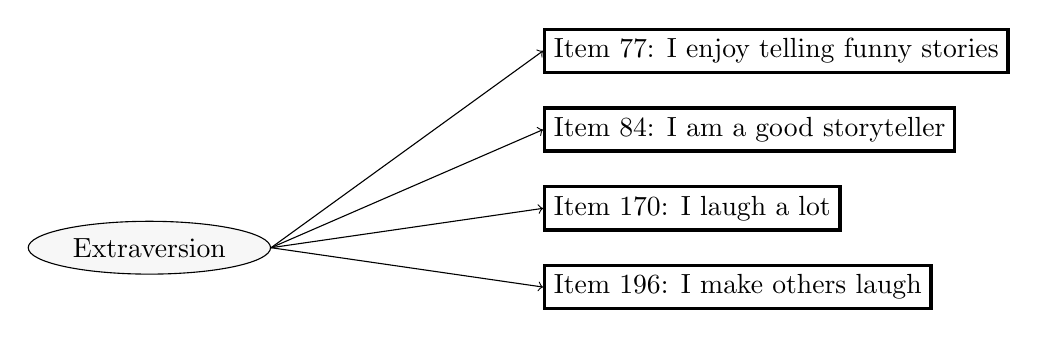
\begin{tikzpicture}[
      squarednode/.style={rectangle, draw=black, very thick, minimum size=5mm},
      arrow/.style = {thick}
    ]
    \usetikzlibrary{shapes.geometric}

    %Nodes
    \node[ellipse, draw,fill=gray!6] at (-1,3) (latent) {Extraversion};
    \node[squarednode,right=2cm of latent,yshift=0.5cm] at (2,5) (Item77) {Item 77: I enjoy telling funny stories}; 
    \node[squarednode,right=2cm of latent,yshift=0.5cm] at (2,4) (Item84) {Item 84: I am a good storyteller};
    \node[squarednode,right=2cm of latent,yshift=0.5cm] at (2,3) (Item170) {Item 170: I laugh a lot};
    \node[squarednode,right=2cm of latent,yshift=0.5cm] at (2,2) (Item196) {Item 196: I make others laugh};
    
    %%Arrows
    \draw[->] (latent.east) -- (Item77.west);
    \draw[->] (latent.east) -- (Item84.west);
    \draw[->] (latent.east) -- (Item170.west);
    \draw[->] (latent.east) -- (Item196.west);
    
    \end{tikzpicture}}
    
\end{frame}
%------------------------------------------------------------------------------%
%
% Slide 54
\begin{frame}{Latent variable scaling Ctd.}

% Latent variables are not observed, thus no inherent scale.
% 
% \vspace{5mm}
% 
% Therefore, set up model such that scale of latent variable is clear. 
% 
% \vspace{5mm}

    \scalebox{0.6}{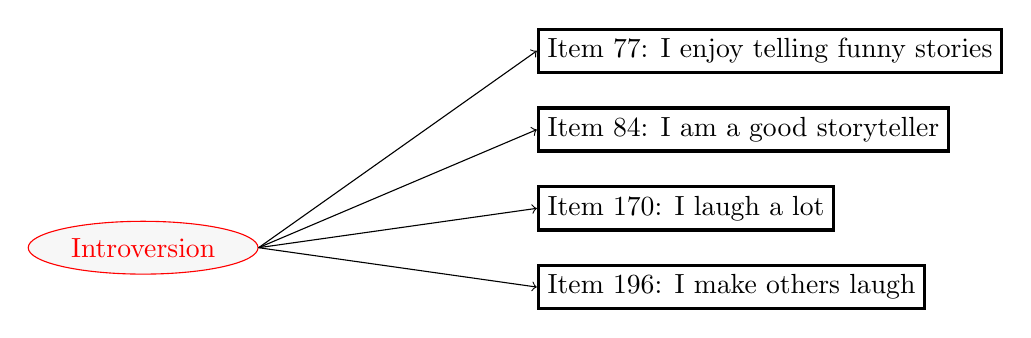
\begin{tikzpicture}[
      squarednode/.style={rectangle, draw=black, very thick, minimum size=5mm},
      arrow/.style = {thick}
    ]
    \usetikzlibrary{shapes.geometric}

    %Nodes
    \node[red, ellipse, draw,fill=gray!6] at (-1,3) (latent) {Introversion};
    \node[squarednode,right=2cm of latent,yshift=0.5cm] at (2,5) (Item77) {Item 77: I enjoy telling funny stories}; 
    \node[squarednode,right=2cm of latent,yshift=0.5cm] at (2,4) (Item84) {Item 84: I am a good storyteller};
    \node[squarednode,right=2cm of latent,yshift=0.5cm] at (2,3) (Item170) {Item 170: I laugh a lot};
    \node[squarednode,right=2cm of latent,yshift=0.5cm] at (2,2) (Item196) {Item 196: I make others laugh};
    
    %%Arrows
    \draw[->] (latent.east) -- (Item77.west);
    \draw[->] (latent.east) -- (Item84.west);
    \draw[->] (latent.east) -- (Item170.west);
    \draw[->] (latent.east) -- (Item196.west);
    
    \end{tikzpicture}}
    
    \vspace{5mm}

    Therefore, set up model such that scale of latent variable is clear.

\end{frame}
%------------------------------------------------------------------------------%
%
% Slide 55
\begin{frame}{Three common ways}

1. Marker-variable method \\
Constrain one of the factor loadings (default).

\vspace{5mm}

2. Reference group method: \\
Constrain the factor variance.

\vspace{5mm}

3. Effect coding:\\
Constrain the average of the loadings. 

\vspace{5mm}

    \scalebox{0.6}{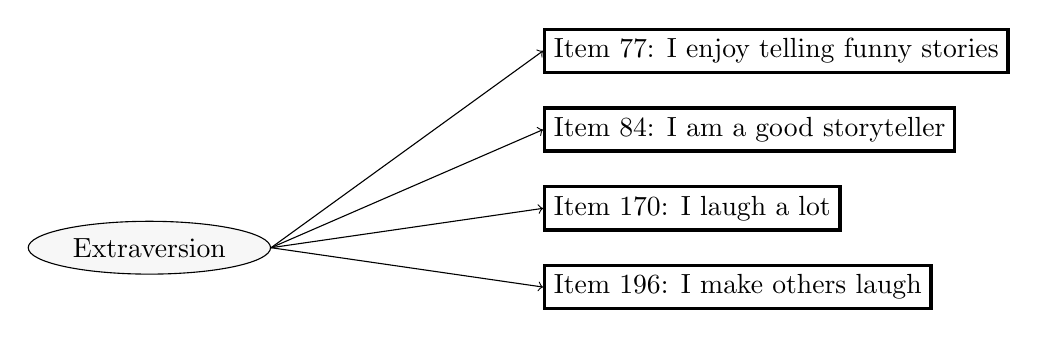
\begin{tikzpicture}[
      squarednode/.style={rectangle, draw=black, very thick, minimum size=5mm},
      arrow/.style = {thick}
    ]
    \usetikzlibrary{shapes.geometric}

    %Nodes
    \node[ellipse, draw,fill=gray!6] at (-1,3) (latent) {Extraversion};
    \node[squarednode,right=2cm of latent,yshift=0.5cm] at (2,5) (Item77) {Item 77: I enjoy telling funny stories}; 
    \node[squarednode,right=2cm of latent,yshift=0.5cm] at (2,4) (Item84) {Item 84: I am a good storyteller};
    \node[squarednode,right=2cm of latent,yshift=0.5cm] at (2,3) (Item170) {Item 170: I laugh a lot};
    \node[squarednode,right=2cm of latent,yshift=0.5cm] at (2,2) (Item196) {Item 196: I make others laugh};
    
    %%Arrows
    \draw[->] (latent.east) -- (Item77.west);
    \draw[->] (latent.east) -- (Item84.west);
    \draw[->] (latent.east) -- (Item170.west);
    \draw[->] (latent.east) -- (Item196.west);
    
    \end{tikzpicture}}
    
\end{frame}
%------------------------------------------------------------------------------%
%
% Slide 56
\begin{frame}{1. Marker-variable method (default)}

    \begin{columns}[T] % align columns
    \begin{column}{.65\textwidth}

        \textbf{Default parameterization:}
        \begin{itemize}
            \item First factor loading constrained at \textcolor{orange}{1}.
            \item Factor mean constrained at \textcolor{orange}{0}.
        \end{itemize} 
        \textbf{Other defaults:}
        \begin{itemize}
            \item Mean of residuals is by definition 0.
            \item Residuals have a loading of 1.
        \end{itemize} 
        \textbf{Estimated:}
        \begin{itemize}
            \item factor variance ($\Psi$), 
            \item `other' factor loadings ($\lambda_2$, $\lambda_3$),
            \item all item intercepts ($\nu_1$, $\nu_2$, $\nu_3$), 
            \item all residual variances ($\epsilon_1$, $\epsilon_2$, $\epsilon_3$).
        \end{itemize}

    \end{column}%
    
    \hfill%
    \begin{column}{.34\textwidth}

            \includegraphics[width=\linewidth,height=\textheight,keepaspectratio]{images/slide56.png}     
     
    \end{column}%

    \end{columns}

\end{frame}
%------------------------------------------------------------------------------%
%
% Slide 58
\begin{frame}[fragile]{1. Default marker-variable method - lavaan}

\begin{knitrout}
\definecolor{shadecolor}{rgb}{0.969, 0.969, 0.969}\color{fgcolor}\begin{kframe}
\begin{alltt}
\hlcom{# Model}
\hldef{model.1CFA} \hlkwb{<-} \hlsng{'
 Extraversion =~ Q77 + Q84 + Q170 + Q196
'}

\hlcom{# Fit model}
\hldef{fit_1CFA} \hlkwb{<-} \hlkwd{cfa}\hldef{(model.1CFA,} \hlkwc{data}\hldef{=data_sapi,}
                \hlkwc{missing}\hldef{=}\hlsng{'fiml'}\hldef{,} \hlkwc{fixed.x}\hldef{=F)}  \hlcom{# use FIML}
\end{alltt}
\end{kframe}
\end{knitrout}

\begin{itemize}
    \item First factor loading constrained at \textcolor{orange}{1}:\\
\begin{verbatim}
Extraversion =~                                     
  Q77               1.000
\end{verbatim}
    \item Factor mean constrained at \textcolor{orange}{0}:\\
\begin{verbatim}
Extraversion      0.000
\end{verbatim}
\end{itemize} 

\end{frame}
%------------------------------------------------------------------------------%
%
% Slide 59
\begin{frame}[fragile]{1. Default marker-variable method - lavaan Ctd}

\begin{knitrout}
\definecolor{shadecolor}{rgb}{0.969, 0.969, 0.969}\color{fgcolor}\begin{kframe}
\begin{alltt}
\hlkwd{parameterEstimates}\hldef{(fit_1CFA)[}\hlnum{1}\hlopt{:}\hlnum{4}\hldef{,}\hlopt{-}\hlkwd{c}\hldef{(}\hlnum{5}\hldef{,}\hlnum{6}\hldef{,}\hlnum{7}\hldef{)]}
\end{alltt}
\begin{verbatim}
##            lhs op  rhs   est ci.lower ci.upper
## 1 Extraversion =~  Q77 1.000    1.000    1.000
## 2 Extraversion =~  Q84 0.708    0.616    0.799
## 3 Extraversion =~ Q170 0.567    0.466    0.668
## 4 Extraversion =~ Q196 0.742    0.640    0.845
\end{verbatim}
\end{kframe}
\end{knitrout}

Factor loading of first indicator fixed to 1. \\
all other loadings are relative to that.

\vspace{5mm}

If reference category changed, other loadings also change. 

\end{frame}
%------------------------------------------------------------------------------%
%
% Slide 60
\begin{frame}{2. Reference-group method}

    \begin{columns}[T] % align columns
    \begin{column}{.65\textwidth}
    
    \textbf{Parameterization:}
        \begin{itemize}
            \item Factor variance constrained at \textcolor{orange}{1}.
            \item Factor mean constrained at \textcolor{orange}{0}.*
        \end{itemize} 
        \textbf{Defaults:}
        \begin{itemize}
            \item Mean of residuals is by definition 0.
            \item Residuals have a loading of 1.
        \end{itemize} 
        \textbf{Estimated:}
        \begin{itemize}
            \item all factor loadings ($\lambda_1$, $\lambda_2$, $\lambda_3$),
            \item all item intercepts ($\nu_1$, $\nu_2$, $\nu_3$), 
            \item all residual variances ($\epsilon_1$, $\epsilon_2$, $\epsilon_3$).
        \end{itemize}
    
    \end{column}%
    
    \hfill%
    \begin{column}{.34\textwidth}
        \includegraphics[width=\linewidth,height=\textheight,keepaspectratio]{images/slide60.png}
    \end{column}%
    \end{columns}
    
    \vspace{5mm}
    
    * In a multi-group model (discussed in another lecture), the mean of the (by default) first group is set to 0 (hence, the name 'reference-group').
    
\end{frame}
%------------------------------------------------------------------------------%
%
\subsection*{Scaling - Part 2}
%------------------------------------------------------------------------------%
%
% Slide 62
\begin{frame}[fragile]{2. Reference-group method - lavaan}

\begin{knitrout}
\definecolor{shadecolor}{rgb}{0.969, 0.969, 0.969}\color{fgcolor}\begin{kframe}
\begin{alltt}
\hlcom{# Model}
\hldef{model.1CFA_RefGr} \hlkwb{<-} \hlsng{'
  # Free first factor loading, using: NA*
  Extraversion =~ NA*Q77 + Q84 + Q170 + Q196
  
  # Set factor variance to 1, using: 1*
  Extraversion ~~ 1*Extraversion
 '}

\hlcom{# Fit model}
\hldef{fit_1CFA_RefGr} \hlkwb{<-} \hlkwd{cfa}\hldef{(model.1CFA_RefGr,} \hlkwc{data}\hldef{=data_sapi,}
                \hlkwc{missing}\hldef{=}\hlsng{'fiml'}\hldef{,} \hlkwc{fixed.x}\hldef{=F)}  \hlcom{# use FIML}
\end{alltt}
\end{kframe}
\end{knitrout}

Shortcut to fix the variances of (all the) latent variables to 1:

\begin{knitrout}
\definecolor{shadecolor}{rgb}{0.969, 0.969, 0.969}\color{fgcolor}\begin{kframe}
\begin{alltt}
\hldef{fit_1CFA_RefGr2} \hlkwb{<-} \hlkwd{cfa}\hldef{(model.1CFA,}    \hlcom{# ! 'original' model !}
                       \hlkwc{std.lv} \hldef{=} \hlnum{TRUE}\hldef{,} \hlcom{# fix variances to 1}
                \hlkwc{data}\hldef{=data_sapi,} \hlkwc{missing}\hldef{=}\hlsng{'fiml'}\hldef{,} \hlkwc{fixed.x}\hldef{=F)}
\end{alltt}
\end{kframe}
\end{knitrout}

% \begin{itemize}
%     \item Factor variance constrained at \textcolor{orange}{1}:\\
% \begin{verbatim}
% Extraversion      1.000
% \end{verbatim}
%     \item Factor mean constrained at \textcolor{orange}{0}:\\
% \begin{verbatim}
% Extraversion      0.000
% \end{verbatim}
% \end{itemize} 

\end{frame}
%------------------------------------------------------------------------------%
%
% Slide 63
\begin{frame}[fragile]{2. Reference-group method - lavaan Ctd}

\begin{knitrout}
\definecolor{shadecolor}{rgb}{0.969, 0.969, 0.969}\color{fgcolor}\begin{kframe}
\begin{alltt}
\hlkwd{parameterEstimates}\hldef{(fit_1CFA_RefGr)[}\hlnum{1}\hlopt{:}\hlnum{4}\hldef{,}\hlopt{-}\hlkwd{c}\hldef{(}\hlnum{5}\hldef{,}\hlnum{6}\hldef{,}\hlnum{7}\hldef{)]}
\end{alltt}
\begin{verbatim}
##            lhs op  rhs   est ci.lower ci.upper
## 1 Extraversion =~  Q77 0.835    0.759    0.910
## 2 Extraversion =~  Q84 0.591    0.520    0.662
## 3 Extraversion =~ Q170 0.473    0.404    0.543
## 4 Extraversion =~ Q196 0.619    0.559    0.680
\end{verbatim}
\begin{alltt}
\hlcom{#parameterEstimates(fit_1CFA_RefGr2)[1:4,-c(5,6,7)]}
\end{alltt}
\end{kframe}
\end{knitrout}

Advantage:\\ 
All factor loadings and scores on standardized metric. 

\end{frame}
%------------------------------------------------------------------------------%
%
% Slide 64
\begin{frame}{Which method to choose?}

% {\centering
%     \includegraphics[width=\linewidth,height=0.5\textwidth,keepaspectratio]{images/slide64.png}      
% }

\begin{columns}[T] % align columns
    \begin{column}{.49\textwidth}
    
    {\centering{1. Marker-variable method}}
    \includegraphics[height=5cm,keepaspectratio]{images/slide56.png}
    
    \end{column}%
    
    \hfill%
    \begin{column}{.49\textwidth}
    
    {\centering{2. Reference-group method}}
        \includegraphics[height=4.35cm,keepaspectratio]{images/slide60.png}
    \end{column}%
    
    \end{columns}
    
Does not matter for substantive conclusions.\\
Sometimes, pragmatic reasons. 

\end{frame}
%------------------------------------------------------------------------------%
%
% Slide 65
\begin{frame}{3. Effects-coding method}

    \begin{columns}[T] % align columns
    \begin{column}{.65\textwidth}
    
    \textbf{Parameterization:}
        \begin{itemize}
            \item Constrain the average of the factor loadings to 1:
            $\frac{1}{3} \sum_{i=1}^3 \lambda_i = 1$. %(hence, sum = 3).
            \item Constrain the average of the item intercepts to 0:
            $\frac{1}{3} \sum_{i=1}^3 \nu_i = 0$.
        \end{itemize} 
        \textbf{Defaults:}
        \begin{itemize}
            \item Mean of residuals is by definition 0.
            \item Residuals have a loading of 1.
        \end{itemize} 
        \textbf{Estimated (subject to the constraints):}
        \begin{itemize}
            \item factor variance ($\Psi$),
            \item factor mean ($\alpha$),
            \item all factor loadings ($\lambda_1$, $\lambda_2$, $\lambda_3$),
            \item all item intercepts ($\nu_1$, $\nu_2$, $\nu_3$), 
            \item all residual variances ($\epsilon_1$, $\epsilon_2$, $\epsilon_3$).
        \end{itemize}
    
    \end{column}%
    
    \hfill%
    \begin{column}{.34\textwidth}
        \includegraphics[width=\linewidth,height=\textheight,keepaspectratio]{images/slide66.png} 
    \end{column}%
    \end{columns}
    
\end{frame}
%------------------------------------------------------------------------------%
%
% Slide 65
\begin{frame}{3. Effects-coding method Ctd}
    
    {\centering
    \includegraphics[height=3cm,keepaspectratio]{images/slide66.png} 
    }
        
Interpretations can be intuitive: 
\begin{itemize}
  \item Factor on similar scale as the indicators.
  \item Factor variance ($\Psi$): average variance of each indicator that can be explained by the factor.
  \item Factor mean ($\alpha$): weighted mean of the indicator means
\end{itemize}
    
\end{frame}
%------------------------------------------------------------------------------%
%
% Slide 66-67
\begin{frame}[fragile]{3. Effects-coding method - lavaan model}

\begin{knitrout}
\definecolor{shadecolor}{rgb}{0.969, 0.969, 0.969}\color{fgcolor}\begin{kframe}
\begin{alltt}
\hlcom{# Model}
\hldef{model.1CFA_EffC} \hlkwb{<-} \hlsng{'
  # Label parameters, such that they can be constrained
  Extraversion =~ lambda1*Q77 + lambda2*Q84 + 
                  lambda3*Q170 + lambda4*Q196
  # intercepts
  Q77  ~ nu1*1
  Q84  ~ nu2*1
  Q170 ~ nu3*1
  Q196 ~ nu4*1
  
  # Constrain average of loadings to 1, i.e., set sum to 4
  lambda1 == 4 - lambda2 - lambda3 - lambda4
  # Constrain average of item intercepts to 0, 
  # i.e., set sum to 0
  nu1 == 0 - nu2 - nu3 - nu4
 '}
\end{alltt}
\end{kframe}
\end{knitrout}

\end{frame}
%------------------------------------------------------------------------------%
%
% Slide 66-67
\begin{frame}[fragile]{3. Effects-coding method - fit lavaan model}

Now, use the lavaan() function:

\vspace{5mm}

\begin{knitrout}
\definecolor{shadecolor}{rgb}{0.969, 0.969, 0.969}\color{fgcolor}\begin{kframe}
\begin{alltt}
\hlcom{# Fit model: Now, use the lavaan() function!}
\hldef{fit_1CFA_EffC} \hlkwb{<-} \hlkwd{lavaan}\hldef{(model.1CFA_EffC,} \hlkwc{data}\hldef{=data_sapi,}
                      \hlkwc{missing}\hldef{=}\hlsng{'fiml'}\hldef{,} \hlkwc{fixed.x}\hldef{=F,}
                      \hlkwc{auto.var} \hldef{=} \hlnum{TRUE}\hldef{,}
                      \hlkwc{auto.fix.first} \hldef{=} \hlnum{FALSE}\hldef{,}
                      \hlkwc{auto.cov.lv.x} \hldef{=} \hlnum{TRUE}\hldef{,}
                      \hlkwc{int.ov.free} \hldef{=} \hlnum{TRUE}\hldef{)}
\end{alltt}
\end{kframe}
\end{knitrout}
% summary(fit_1CFA_EffC)

\end{frame}
%------------------------------------------------------------------------------%
%
% Slide 67
\begin{frame}[fragile]{3. Effects-coding method - lavaan output}

\begin{itemize}
    \item Constrain the average of the factor loadings to 1:
    $\frac{1}{4} \sum_{i=1}^4 \lambda_i = 1$. \\ %(hence, sum = 3).
\begin{knitrout}
\definecolor{shadecolor}{rgb}{0.969, 0.969, 0.969}\color{fgcolor}\begin{kframe}
\begin{alltt}
\hlkwd{parameterEstimates}\hldef{(fit_1CFA_EffC)[}\hlnum{1}\hlopt{:}\hlnum{4}\hldef{,}\hlnum{1}\hlopt{:}\hlnum{5}\hldef{]}
\end{alltt}
\begin{verbatim}
##            lhs op  rhs   label   est
## 1 Extraversion =~  Q77 lambda1 1.197
## 2 Extraversion =~  Q84 lambda2 1.027
## 3 Extraversion =~ Q170 lambda3 0.879
## 4 Extraversion =~ Q196 lambda4 0.898
\end{verbatim}
\end{kframe}
\end{knitrout}
    \item Constrain the average of the item intercepts to 0:
    $\frac{1}{4} \sum_{i=1}^4 \nu_i = 0$.\\
\begin{knitrout}
\definecolor{shadecolor}{rgb}{0.969, 0.969, 0.969}\color{fgcolor}\begin{kframe}
\begin{alltt}
\hlkwd{parameterEstimates}\hldef{(fit_1CFA_EffC)[}\hlnum{5}\hlopt{:}\hlnum{8}\hldef{,}\hlnum{1}\hlopt{:}\hlnum{5}\hldef{]}
\end{alltt}
\begin{verbatim}
##    lhs op rhs label    est
## 5  Q77 ~1       nu1 -0.765
## 6  Q84 ~1       nu2 -0.521
## 7 Q170 ~1       nu3  0.738
## 8 Q196 ~1       nu4  0.548
\end{verbatim}
\end{kframe}
\end{knitrout}
\end{itemize}

\end{frame}
%------------------------------------------------------------------------------%
%
%------------------------------------------------------------------------------%
\section{The end}
%------------------------------------------------------------------------------%
%
%------------------------------------------------------------------------------%
%
\begin{frame}{Summary}

  \begin{itemize}
      \item EFA and CFA
      \item Scaling
  \end{itemize}

\end{frame}
% %------------------------------------------------------------------------------%
% %
% \begin{frame}{Take home message}
% \begin{itemize}
% \item{} 
%   \begin{itemize}
%   \item{}
%   \item{}
%   \end{itemize}
% \item{}
% \end{itemize}
% \end{frame}
%------------------------------------------------------------------------------%
%
\begin{frame}{Thanks \& How to proceed}

Thanks for listening!

\vspace*{5mm}

Are there any questions?\\
\begin{itemize}
  \item Ask fellow participant on course platform.
  \item Ask teacher during Q\&A (or via course platform).
  \item See if making the lab exercises help.
  \item Check the lavaan tutorial: e.g., \url{https://lavaan.ugent.be/tutorial/index.html}.
  \item Do not forget that Google is your best friend :-).
\end{itemize}

\vspace*{5mm}

You can start working on the lab exercises.

\end{frame}
%------------------------------------------------------------------------------%
%
%------------------------------------------------------------------------------%
%
\section{Extra}

% Slide extra 1
\begin{frame}
	
	\begin{center}
		\Huge{Extra:}
		
		\large{Sample size}
	\end{center}
	
	\vspace*{15mm}
	
based on https://www.theanalysisfactor.com/sample-size-needed-for-factor-analysis/

\end{frame}
%
% Slide extra 2
\begin{frame}{Sample Size Rules of Thumb - total sample size}
	
Some authors use a criterion based on the total sample size:
~\\

\begin{itemize}
\item 100 subjects = sufficient if clear structure; more is better \\ (Kline, 1994).
\item 100 subjects = poor; 300 = good; 1000+ = excellent \\ (Comrey \& Lee, 1992).
\item 300 subjects, though fewer works if correlations are high among variables \\ (Tabachnik \& Fidell, 2001).
\end{itemize}

\end{frame}
%
% Slide extra 3
\begin{frame}{Sample Size Rules of Thumb - ratio cases vs variables}
	
Others base it on a ratio of the number of cases to the number of variables involved in the factor analysis:
~\\

\begin{itemize}
\item 10-15 subjects per variable (Pett, Lackey, \& Sullivan).
\item 10 subjects per variable (Nunnally, 1978).
\item 5 subjects per variable or 100 subjects, whichever is larger \\ (Hatcher, 1994).
\item 2 subjects per variable (Kline, 1994).
\end{itemize}

\end{frame}
%
% Slide extra 4
\begin{frame}{Sample Size Rules of Thumb - ratio cases vs factors}
	
And then others base it on a ratio of cases to the number of factors:
~\\

\begin{itemize}
\item 20 subjects per factor (Arrindel \& van der Ende, 1985).
\end{itemize}

\end{frame}


% Slide 20
\begin{frame}
	
	\begin{center}
		\Huge{Extra:}
		
		\large{Categorical/Ordinal or continuous indicators?}
	\end{center}
	
	\vspace*{15mm}
	
	Note: in cfa() you can, for example use `ordered = TRUE' for  endogenous variable.\\
	Default then: estimator = "WLSMV".
	
	\vspace*{15mm}
	
	More information on: https://lavaan.ugent.be/tutorial/cat.html
	
\end{frame}

% Slide 21
\begin{frame}
	
	\includegraphics[width=\linewidth,height=\textheight,keepaspectratio]{images/slide21.png}
	
\end{frame}

% Slide 22 - not needed?
% TO DO?

% SLIDE 23
\begin{frame}{Remark!}
	
Do NOT use a $\chi^2$ test or IC (AIC or BIC) \\
to compare categorical and continuous models:

\vspace{5mm}

\begin{itemize}
	\item Obviously not nested (so, no $\chi^2$ test anyway).
	\item AND likelihoods of categorical and continuous indicator models are incomparable!
\end{itemize}
	
	\vspace{5mm}
	
	Note: $\chi^2$ test and IC are based on (log) likelihood (= fit).
	
\end{frame}

% Slide 24 not there/blank

%% Slide 25
%\begin{frame}
%	
%	\includegraphics[width=\linewidth,height=\textheight,keepaspectratio]{images/slide25.png}
%	
%\end{frame}
%
%% Slide 26 - NOT NEEDED


% Slide 27
\begin{frame}{Interesting Reading}
	
	https://lavaan.ugent.be/tutorial/cat.html
	
	\vspace{5mm}
	
	Muthén, B. (1984). A general structural equation model with dichotomous, ordered categorical, and continuous latent variable indicators. Psychometrica, 49(1), 115-132.
	
	\vspace{5mm}
	
	Rhemtulla, M., Brosseau-Liard, P.É., \& Savalei, V. (2012). When can categorical variables be treated as continuous? A comparison of robust continuous and categorical SEM estimation methods under suboptimal conditions. Psychological Methods, 17(3), 354-373. 
	
	\vspace{5mm}
	
	Sventina, D., Rutkowski, D. (2020). Multiple group invariance with categorical outcomes using updated guidelines: an illustration using Mplus and the lavaan/semtools packages. Structural Equational Modelling: A Multidisciplinary Journal, 27(1), 111-130

\end{frame}


%------------------------------------------------------------------------------%
%
%------------------------------------------------------------------------------%
%
\end{document}





